\documentclass[a4paper,12pt]{report}


\usepackage[protrusion=true,expansion=true]{microtype}

\usepackage[utf8]{inputenc}   
\usepackage[T1]{fontenc}
\usepackage[french]{babel}  
\usepackage[pdftex]{graphicx}
\usepackage{indentfirst}

\usepackage{pdfpages}

\usepackage{lettrine} % The lettrine is the first enlarged letter at the beginning of the text
%\usepackage[sc]{mathpazo} % Use the Palatino font
%\usepackage[condensed,math]{iwona} %////////////////
%\usepackage{inconsolata}
%\renewcommand*\familydefault{\ttdefault}
%\usepackage{kpfonts}
%\usepackage[scaled=1.05,proportional,lightcondensed]{zlmtt}
%\usepackage[default]{comfortaa}
%\usepackage[default]{gfsneohellenic} %////////////////
%\usepackage{ascii}
%\usepackage[default]{comfortaa}
%\usepackage{lmodern}
%\usepackage{mathpazo}
%\usepackage{kpfonts} %////////////
%\usepackage{mathptmx}
%\usepackage{times,mtpro2}
%\usepackage{stix}
%\usepackage{txfonts}
%\usepackage{newtxtext,newtxmath}
%\usepackage{libertine} 
%\usepackage[libertine]{newtxmath}
%\usepackage[scaled=0.85]{luximono}
%\usepackage{arev}
%\usepackage[default]{cantarell} %% Use option "defaultsans" to use cantarell as sans serif only 
%\usepackage{DejaVuSans} %///////////////////:
%\usepackage{PTSansCaption} 
%\renewcommand*\familydefault{\sfdefault} %% Only if the base font of the document is to be sans serif
%\usepackage{venturisold}
%\usepackage{tgschola} %//////////////////////
\usepackage[math]{kurier}
%\usepackage[avantgarde]{quotchap}
% \usepackage[sfdefault,condensed]{cabin}

\usepackage{tabularx}

\usepackage{pgf,pgfarrows,pgfnodes,pgfautomata,pgfheaps,pgfshade}
\usepackage{verbatim}
\usepackage[hang, small,labelfont=bf,up,textfont=it,up]{caption} % Custom captions under/above floats in tables or figures
%\usepackage[colorlinks=true,linkcolor=blue]{hyperref} % For hyperlinks in the PDF

\definecolor{color1}{RGB}{56,115,178}
\definecolor{color2}{RGB}{115,115,115}

\usepackage[pdftex=true,hyperindex=true,colorlinks=true,linkcolor=color1]{hyperref}

%\usepackage{paralist} % Used for the compactitem environment which makes bullet points with less space between them
\usepackage{abstract} % Allows abstract customization
\renewcommand{\abstractnamefont}{\normalfont\bfseries} % Set the "Abstract" text to bold
\renewcommand{\abstracttextfont}{\normalfont\small\itshape} % Set the abstract itself to small italic text

%Options: Sonny, Lenny, Glenn, Conny, Rejne, Bjarne, Bjornstrup
\usepackage[Lenny]{fncychap}



\usepackage{verbatim}
\usepackage{fancyhdr}

\usepackage{setspace}
\usepackage{numprint}
\usepackage{graphicx}
%preamble
\usepackage[nottoc]{tocbibind}

\frenchbsetup{StandardLists=true} % à inclure si on utilise \usepackage[french]{babel}
\usepackage{enumitem}

\usepackage{amsmath,amsfonts,amssymb}

\pagestyle{fancy}

%\linespread{1.5}




\usepackage[french]{algorithm2e}
%\usepackage{algpseudocode,algorithm}
%\floatname{algorithm}{Procedure}
%\renewcommand{\algorithmicrequire}{\textbf{Input:}}
%\renewcommand{\algorithmicensure}{\textbf{Output:}}
%\usepackage{setspace}


\usepackage{titlesec} % Allows customization of titles
%\renewcommand\thesection{\Roman{section}} % Roman numerals for the sections
%\renewcommand\thesubsection{\Roman{subsection}} % Roman numerals for subsections
%\titleformat{\chapter}[farme]{\scshape\huge\bfseries\bf}{\chaptertitlename\ \thechapter}{2em}{} % Change the look of the section titles
%\titleformat{\chapter}[block]{\scshape\bfseries}{}{}{}




%\usepackage{pslatex}



%\usepackage{pifont}
\usepackage{color}
\usepackage{colortbl}
\usepackage{listings}
\usepackage{listingsutf8}

\usepackage[french]{minitoc}

\usepackage{multirow}
%\usepackage{marvosym}
%\usepackage{textcomp}
\usepackage{lastpage}


%\usepackage{nopageno}
%\usepackage{slantsc}
%\usepackage{array}
%\usepackage{amsmath}


%\usepackage{lipsum}





%\nomtcrule
%\renewcommand{\ptctitle}{\scshape}
%\tightmtctrue
%\nomtcpagenumbers




\titleformat{\section}[block]{\Large\scshape\bfseries}{\thesection.}{1em}{} % Change the look of the section titles
\titleformat{\subsection}[block]{\large\scshape\bfseries}{\thesubsection.}{2em}{} % Change the look of the section titles
\titleformat{\subsubsection}[block]{\normalsize\scshape\bfseries}{\thesubsubsection.}{3em}{}
% % % % % % % % % % % % % % % % % % % % % % % % % %
%\pagestyle{empty}
%\setlength{\textwidth}{7in}
%\setlength{\textheight}{9.125in}
%\setlength{\columnsep}{0.5in}
%\setlength{\topmargin}{-0.8in}
%\setlength{\oddsidemargin}{-0.25in}
%\setlength{\parindent}{5ex}   

% % % % % % % % % % % % % % % % % % % % % % % % % % %
\setlength{\hoffset}{-0pt}    %//////////////////////////    
\setlength{\oddsidemargin}{15pt} % Marge gauche sur pages impaires %/////////////////////
%\setlength{\evensidemargin}{9pt} % Marge gauche sur pages paires
\setlength{\marginparwidth}{0pt} % Largeur de note dans la marge
\setlength{\textwidth}{420pt} % Largeur de la zone de texte (17cm) %//////////////////
%\setlength{\voffset}{-18pt} % Bon pour DOS
\setlength{\marginparsep}{0pt} % Séparation de la marge
\setlength{\headwidth}{420pt}
%\setlength{\topmargin}{0pt} % Pas de marge en haut
%\setlength{\headheight}{13pt} % Haut de page
%\setlength{\headsep}{10pt} % Entre le haut de page et le texte
%\setlength{\footskip}{27pt} % Bas de page + séparation
%\setlength{\textheight}{615pt} % Hauteur de la zone de texte (25cm) %/////////////
      

%\title{Gestion des consommations d’énergie dans\\ les Clouds Computing}
\title{\vspace{-15mm}\fontsize{24pt}{10pt}\selectfont\textbf{Gestion de la consommation d’énergie\\ dans le Cloud Computing}} % Article title
%\author{ \textit{\textbf{YAGOUBI Djamel Eddine}} }
%\date{1 Avril 2014}
\author{
\large
\textsc{YAGOUBI Djamel Edine}\thanks{YAGOUBI Djamel Edine avec \textbf{\LaTeX}}\\[2mm] % Your name
\normalsize \textsc{Université D'Oran} \\ % Your institution
\normalsize \href{mailto:yagoubi.djamel@gmail.com}{Yagoubi.djamel@gmail.com} % Your email address
\vspace{-5mm}
}
\date{1 Avril 2014}


\setcounter{secnumdepth}{3}
\setcounter{tocdepth}{3}

\begin{document}
 
%\pagestyle{headings} 
%\fancyhead[R]{}
%\fancyfoot[]{\leftmark }
%\pagestyle{fancy}



%\renewcommand{\footrulewidth}{1pt}

% % % % % % % % % % % % % % % % % % % % % % % % % % % % %

\fancyhead{}

\renewcommand{\headrule}
{%
\hrule width\headwidth height\headrulewidth \vskip-\headrulewidth}

\fancyhead[EL,OL]
{\textsl{\rightmark}}
\fancyhead[ER,OR]
{\subsectionmark{\leftmark}}

\fancyfoot{} 
\fancyfoot[RO,RE]
{{\bfseries\ Page}
{\textbar} 
\bfseries\textbf{\thepage}
}

\fancyfoot[LO,LE]
{\sectionmark}

\fancyfoot[L]{\tiny  Réalisé par {\bf \footnotesize \sc YAGOUBI Djamel Edine} à l’aide du logiciel de composition typographique \scriptsize \LaTeX}

\renewcommand{\footrule}{{%
\vskip-\footruleskip\vskip-\footrulewidth
\hrule  \headwidth  \footrulewidth  \vskip \footruleskip}}

% % % % % % % % % % % % % % % % % % % % % % % % % % % % %



%\maketitle


\includepdf[pages = -]{PageDeGard/PageDeGard}



\pagenumbering{Roman}



\dominitoc

\thispagestyle{empty}
\begin{center}
\resizebox{!}{8mm}{\bf \scshape \selectfont Dédicace}\\
\end{center}

\vspace{20mm}


\begin{flushright}

Je dédie ce modeste travail à mes très chers\\



\end{flushright} 


%\addcontentsline{toc}{chapter}{Dédicace}
\clearpage
\thispagestyle{empty}
\begin{center}
\resizebox{!}{8mm}{\bf \scshape \selectfont Remerciments}\\
\end{center}

\vspace{20mm}


%\begin{flushright}
En préambule à ce mémoire je remercie ALLAH qui m’aide et me donne la patience et le courage pour accomplir ce modeste travail.\bigskip

Je tiens à exprimer mes sincères remerciements et toute mon gratitude à mon encadreur le Professeur G. Belalem et à mon co-encadreur Mlle D. Djouhra  pour avoir accepté d’encadrer ce mémoire. J’aimerai leur adresser mes plus vifs remerciements pour tous leurs dynamismes, conseils, disponibilités, suivis, et leurs compétences scientifiques que nous avons pu apprécier tout au long de cette année.\bigskip

Mes vifs remerciements vont aussi au jury, l’honorable Présidente Mlle M. Bourenane et les honorables membres Mme F. Z. Bellounar et Mr N. Lachachi pour l’intérêt qu’ils m’ont porté à mes recherches, en acceptant d’examiner mon travail et de l’enrichir par leurs propositions.\bigskip

Je tiens aussi à remercier les enseignants qui m’ont aidé et soutenu durant toutes mes éducations.\bigskip

Mes derniers remerciements vont à ma famille et notamment à mes parents, mes amis, car sans leurs constants soutiens et leurs encouragements, je n’aurai pas pu mener à bien ce mémoire.\bigskip

Merci infiniment encore à tous.

%\end{flushright} 
%\addcontentsline{toc}{chapter}{Remerciements}
\clearpage

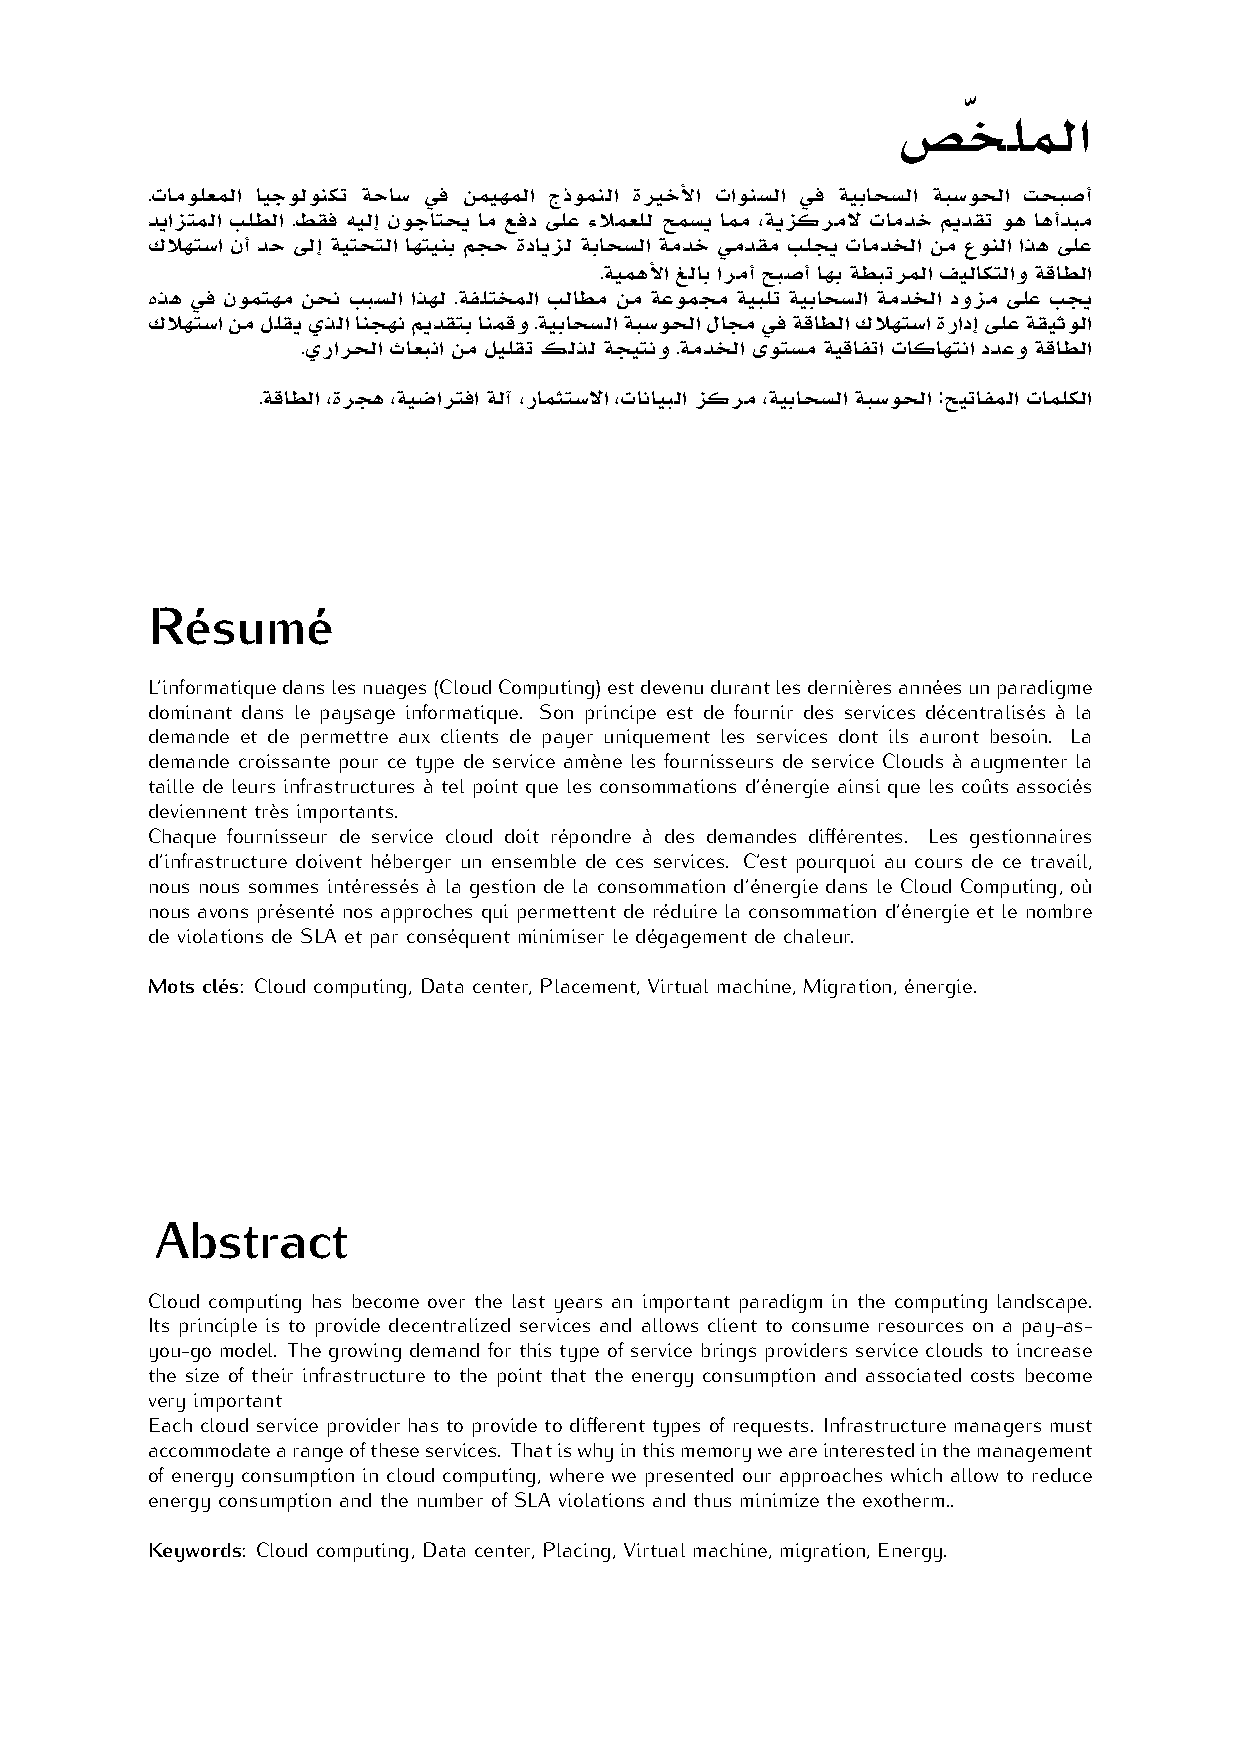
\includepdf[pages = -]{Abstract/Abstract}

\clearpage



\thispagestyle{empty}
\begin{center}
\resizebox{!}{8mm}{\bf \scshape \selectfont Introduction générale}\\
\end{center}
%\lhead{\normalsize \bf \selectfont Introduction générale}
\vspace{20mm}

%\lipsum[1-3]
\begin{onehalfspace}
\lettrine[nindent=1em,lines=3]{L}'informatique dans les nuages (cloud computing en anglais) s’est imposée ces dernières années comme un paradigme majeur d’utilisation des infrastructures informatiques. Celui-ci répond à des besoins et demandes croissantes en terme de disponibilité et flexibilité. 
Le développement remarquable du Cloud Computing, ces dernières années, suscite de plus en plus l’intérêt des différents utilisateurs de l’Internet et de l’informatique qui cherchent à profiter au mieux des services et des applications disponibles en ligne à travers le Web en mode services à la demande et facturation à l’usage.\\

L’approche du Cloud Computing s’appuie principalement sur le concept de virtualisation. Ce concept est un ensemble de techniques permettant de faire fonctionner sur une seule machine plusieurs systèmes d’exploitation et/ou plusieurs applications, isolés les uns des autres. Un Cloud est constitué d’un ensemble de machines virtuelles qui utilisent la même infrastructure physique.\\

La croissance des deux côtés de l’offre et de la demande rend le problème de la consommation d’énergie plus complexe, sophistiqué dans un environnement Cloud. Les demandes cumulées sur une seule machine virtuelle ou en général sur un seul Data Center mènent à la saturation. Ces derniers ne pourront plus satisfaire les demandes des utilisateurs. D’autre part les besoins en ressources des applications peuvent aller au-delà de ce qui est disponible dans un Cloud.\\

La consommation électrique des centres de données (data centers en anglais) dans le monde a été estimée pour 2010 entre 1.1\% et 1.5\% de la consommation électrique globale. Même si cela parait peu en proportion, cette consommation d’énergie représente plus de 200 milliards de kilowatt-heure \cite{ref48}. Cette consommation d’énergie est en croissance permanente au fil des années. Elle était estimée à 12\% par an en 2007 par l’U.S Environmental Protection Agency pour atteindre un coût de l’électricité utilisée par les serveurs des data centers estimé de 7.4 milliards de dollars \cite{EPA_2007}.\\

Dans ce travail, l’objectif visé est de proposer une stratégie basée sur la migration des machines virtuelles, en appliquant des méthodes et des algorithmes. Notre politique de migration des machines virtuelles vise à optimiser la consommation d’énergie.\\

{\scshape\bfseries Organisation du mémoire}\\

Le présent mémoire est structuré autour de quatre principaux chapitres qui se résument comme suit :
\begin{description}
\item[Chapitre 1 :] Dans le premier chapitre, nous présenterons le problème de la consommation d’énergie des data center et son impact énergétique.
\item[Chapitre 2 :] Le second chapitre présentera quelques différentes techniques d’optimisations d’énergie et les principaux travaux de recherches qui ont été proposés dans la littérature.
\item[Chapitre 3 :] Le troisième chapitre sera réservé à la description détaillée de la conception de la stratégie utilisée ainsi que des services que nous avons proposés. Cette conception se fera à l’aide de formules, d’algorithmes et de diagrammes UML.
\item[Chapitre 4 :] Ce dernier chapitre présentera les étapes de l’implémentation de l’approche proposée. Nous y détaillerons la réalisation de certaines fonctionnalités ainsi que l’étude d’évaluation de cette stratégie. Les résultats d’expérimentation seront interprétés.
\end{description}

Enfin, un ensemble de perspectives viendra clore notre travail.

\end{onehalfspace}



\tableofcontents


\pagenumbering{arabic}
%\doublespace
\ChNumVar{\fontsize{76}{80}\usefont{OT1}{pzc}{m}{n}\selectfont}

\ChTitleVar{\scshape \raggedleft \LARGE  \bfseries}


\chapter{Consommations d'énergie des data centers} % Main chapter title %
\vspace{3cm}
\minitoc
%\vspace{3cm}
% \begin{center}
%\resizebox{!}{6mm}{\bf \fontfamily{lmss}\selectfont Consommations d'énergie au niveau des data centers}\\
%\end{center}
%\lhead{\normalsize \bf \fontfamily{lmss}\selectfont \@nomChap}

\clearpage



\label{Chapitre1} % For referencing the chapter elsewhere, use \ref{Chapter1} 

%\lhead{Chapitre 1. \emph{Consommations d’énergie}} % This is for the header on each page - perhaps a shortened title




\section{Introduction}
\begin{onehalfspace}
\paragraph{}\lettrine[nindent=1em,lines=3]{L}es énergies fossiles (pétrole, gaz, charbon) ont façonné le monde d’aujourd’hui. Elles sont à l’origine de la révolution industrielle et du développement des transports et ont modelé l’organisation sociale et économique actuelle de l’humanité. Les stocks de pétrole, de gaz et de charbon seront vides d’ici quelques décennies et ne se reconstitueront pas avant plusieurs centaines de millions d’années \cite{WEB46}. Bon gré ou malgré, nous n’avons donc pas d'autres choix que de tendre vers plus de sobriété énergétique, le temps de trouver des alternatives viables aux énergies fossiles. D’autant que l’exploitation intensive de ces ressources carbonées a considérablement augmenté l’effet de serre ces 50 dernières années entraînant un dérèglement climatique global. Ce dérèglement met en danger la survie de l’humanité, notamment en accélérant l’écroulement de la biodiversité.
\paragraph{}Les problèmes liés aux émissions de dioxyde de carbone et à l’énergie font de plus en plus souvent la une des journaux internationaux. Les gouvernements, les associations à but non lucratif et les entreprises réalisent désormais des enquêtes régulières afin d’analyser leur émissions du gaz CO2. Leur objectif est de mesurer l’incidence de leurs activités sur le réchauffement climatique et d’élaborer des plans d’action visant à réduire leurs émissions de dioxyde de carbone.

\end{onehalfspace}
\section{Définition des data centers}
\begin{onehalfspace}
Le data center est un terme anglais qui est employé par les professionnels de l’informatique. Un data center est un bâtiment spécialement conçu pour héberger des équipements informatiques. Ces bâtiments sont découpés en plusieurs salles qu’on appelle des salles blanches. Les grandes entreprises disposent souvent de plusieurs data center pour héberger leurs serveurs. Cependant, de nombreux centre de données sont mutualisés et ils hébergent des serveurs de différents clients.

\end{onehalfspace}
\section{L'impact énergétique des data centers}
\begin{onehalfspace}
L'alimentation électrique est un aspect stratégique pour un cloud data center : sans électricité en quantité suffisante, un data center ne peut pas fonctionner. C'est pour cette raison que les data centers sont construits dans des zones où les infrastructures électriques sont importantes.\medskip 

La consommation d'énergie des salles serveurs ne cesse d'augmenter pour répondre aux besoins notamment des services web. La consommation électrique des data centers a doublé en 5 ans et les études montrent que la tendance s'accélère.\medskip 

La direction informatique se retrouve ainsi au centre de nouveaux enjeux: enjeux financiers comme source de réduction des coûts, enjeux environnementaux en participant à la réduction des émissions de CO$_{2}$. \medskip 

La part de la facture électrique représente 10\% du coût de fonctionnement d'un centre de données. Elle pourrait s'élever très rapidement à 50\% en absence des changements \cite{WEB1}.\medskip \\
Selon une étude IDC, pour 1\$ investit dans le hardware, 1\$ d'énergie sera dépensé \cite{WEB1}.\medskip 

Ces centres qui regroupent les serveurs où sont stockées les données informatiques, sont de véritables gouffres énergétiques. Selon Dalkia\footnote{Dalkia est une entreprise spécialisée dans les services énergétiques, filiale de Veolia Environnement à 66\% et d'Électricité de France à 34\%. Son siège social est situé à Saint-André-lez-Lille, en France.}, un data center de 10.000 $m^{2}$ consomme autant d'énergie qu'une ville de 50.000 habitants.\medskip 

D'après une étude de l'Université de Standford, les quelques 500.000 data centers  existants dans le monde consomment environ 30 milliards de watts d'électricité par an, soit l'équivalent de la production de 30 centrales nucléaires \cite{ref6}.\medskip 

L'énergie dépensée par les centres de stockage des données informatiques est equivalente à 1,5\% de la consommation électrique mondiale. Les data centers seraient également responsables de 2\% des émissions mondiales de CO$_{2}$, soit autant que le trafic aérien mondial.\medskip 

Le poids de la consommation d'énergie des data centers est encore plus important dans les pays développés. selon France Culture\footnote{France Culture est la chaîne de radio culturelle nationale publique française du groupe Radio France.}, en France les data centers consomment 9\% de l’électricité du pays. Les statistiques montrent que le  premier data center construit par Facebook en Europe consomme à lui seul 1\% de l’énergie suédoise.\medskip 

Selon un rapport de l'EPA\footnote{Environmental Protection Agency, Agence américaine de protection de l'environnement \cite{ref3}}, les data centers implantés aux Etats-Unis ont consommé 61 milliards de kilowatt/heures d'électricité en 2006. Ce chiffre représente 1,5 \% de toute l'électricité consommée aux Etats-Unis et un coût de 4,5 milliards de dollars. Les data centers ont été identifiés comme l'un des consommateurs d'énergie qui connaît la croissance la plus rapide. L'EPA exige que le secteur public développe des stratégies pour améliorer l'efficacité énergétique de ses data centers et a fixé un objectif d'amélioration de 20 \% \cite{ref3}. Les data centers du secteur privé, quant à eux, pourraient bien être contraints de respecter sous peu des limites d'émissions de CO$_{2}$.\medskip 
%Les 15 pays qui étaient membres de l’UE avant 2004 se sont engagés à respecter les principes du Protocole de Kyoto. Ils ont convenu de réduire leurs émissions combinées de gaz à effet de serre de 8 \% par rapport à leur niveau de 1990 d’ici 2012(\textit{European Environment Agency, Greenhouse Gas Emission Trends and Projections in Europe 2008, EEA Report No. 5, 2008}). En outre, la Commission Européenne a rédigé un Code de conduite pour les datacenters européens, qui se présente sous la forme d’un ensemble de mesures volontaires d’amélioration de l’efficacité conçu pour définir des normes minimales qui serviront de base à l’établissement d’une réglementation plus contraignante à l’avenir. Son objectif ultime est d’améliorer de 30 \% l’efficacité énergétique moyenne des datacenters.\\

La croissance du secteur étant très importante en raison du développement d'Internet sur appareils mobiles et de l'augmentation des besoins de stockage des entreprises. La demande énergétique liée au data centers va continuer à augmenter fortement.
\end{onehalfspace}
\section{Pourquoi les data centers consomment autant d'énergie ?}
\begin{onehalfspace}
La consommation d’énergie conséquente des data centers s’explique par plusieurs raisons. D'une par, les serveurs de stockage ne peuvent pratiquement jamais être arrêtés pour ne pas perdre les données confiées par les clients des data centers. Ils fonctionnent donc 24 heures sur 24, tous les jours de l'année.
\medskip 

De plus, ces serveurs sont des appareils électroniques de grande taille qui produisent énormément de chaleur. Leur bon fonctionnement est assuré par des systèmes de climatisation très énergivores.\medskip 

Enfin, pour ne pas perdre de données lors d'éventuelles coupures d'électricité, les data centers sont équipés de générateurs de secours fonctionnant au fioul (émetteurs de CO$_{2}$), voire de batteries, qui contribuent à accentuer leur dépense énergétique.
\end{onehalfspace}
\section{Pourquoi réduire la consommation ?}
\begin{onehalfspace}
Suivant la courbe de progression de la performance de calcul \cite{ref2}, la consommation d’énergie des data centers n’a cessé de croître ces dernières années. %\textbf{Cependant, de la même manière que pour les processeurs, nous allons heurter le mur de la consommation. Lorsque le temps était à la course à la miniaturisation il est apparu que la densité de chaleur générée par le composant imposait une contrainte forte sur la densité des transistors. Un parallèle peut être fait avec les clusters et la consommation d'électricité qu'ils génèrent.}\medskip 

Ainsi, les clusters ont augmenté leur nombre de serveurs en même temps que leur puissance. Ce qui nous amène à faire des prédictions pour le futur de la consommation des data centers, qui sont du même ordre que le mur de la miniaturisation des composants. En effet, la miniaturisation croissante des processeurs a dû ralentir le fait de la dissipation de la chaleur insuffisante, et a amené les constructeurs à changer leurs architectures en augmentant le nombre de processeurs ou de cœurs. Si on prévoit la consommation électrique des superordinateurs du top500 \cite{WEB5} en supposant qu'elle croît de façon constante, on arrivera à des clusters d'une consommation de plusieurs centaines de mégawatts ! ce qui nécessite d'avoir un réacteur nucléaire pour alimenter ces supercalculateurs.\medskip 

Il est donc nécessaire de réduire cette consommation par des moyens permettant à la fois de réduire l’énergie demandée et de garder un niveau acceptable de performance. Eteindre systématiquement la moitié des serveurs entrainant  la  réduction de la consommation d’énergie, ça n’est évidemment pas une solution fiable. Ajoutons à cela l’impact environnemental des data center. Décentraliser les opérations locales réduit la consommation d’énergie et l’émission du gaz CO$_{2}$, cela en délocalisant les applications vers des serveurs plus efficaces énergétiquement. Selon un rapport de Greenpeace \cite{WEB4}, la  consommation d’énergie globale des data centers était responsable en 2007 de 116 tonnes de dioxyde de carbone (MtCO2). Ce même rapport estime que ces mêmes émissions pourraient doubler d’ici  2020 pour atteindre 257 MtCO$_{2}$.\medskip

La consommation d’énergie des serveurs n’est pas en effet la seule source d’émission du gaz CO$_{2}$. Il faut aussi prendre en compte le cycle de vie complet d’un serveur, depuis le moment où le serveur est construit jusqu’à son démantèlement. Un serveur sera responsable de plus d’émission du gaz CO2  que sa consommation d’électricité \cite{WEB46}.\medskip 

Enfin, le coût d'électricité de l'exploitation d'un data center peut rapidement devenir important, jusqu’à ce que la consommation d'électricité sur plusieurs années revienne au même prix qu'acheter ce même data center.\medskip 

Que ce soit donc pour des raisons économiques, environnementales ou tout simplement pratiques,
il est intéressant, voire dans certains cas nécessaire, de réduire la consommation énergétique des clouds. Cependant, comme nous allons le voir par la suite, cela ne peut pas se faire de
n'importe quelle façon.
\end{onehalfspace}
\section{Le Power Usage Effectiveness (PUE)}
\subsection{Le PUE : c'est quoi ?}
\begin{onehalfspace}
Le PUE est un indicateur mis au point par le Green Grid pour mesurer l'efficacité énergétique d'un data center. Il est calculé en divisant le total de l'énergie consommée par le data center par le total de l'énergie utilisée par les équipements informatiques (serveur, stockage, réseau). En moyenne les data center français ont un PUE de 2,5 ce qui signifie que pour 1 Watt consommé par l'équipement informatique, il en faut 2,5 Watt à l'entrée du data center. \\
Sans être un indicateur suffisant pour déterminer l'efficience d'un data center, il n'en demeure pas moins qu'un indicateur universellement reconnu \cite{WEB7}.
\end{onehalfspace}
\subsection{Faut-il choisir entre disponibilité du data center et PUE ?}
\begin{onehalfspace}
Les équipements informatiques sont hébergés dans un data center disposant d’une infrastructure complexe (onduleurs, batteries, groupes électrogènes , climatisations, …) destinée à maximiser le taux de disponibilité des équipements qu’il héberge. La norme TIER définie par l’UPTIME Institute \footnote{The Uptime Institute, association américaine, a défini en 1995 une norme permettant d’analyser les topologies mises en œuvre et de délivrer une certification. Cette norme décrit quatre topologies d’infrastructure de sites dont les niveaux croissants d’éléments et de chemins de distribution redondants servent de base de comparaison.} classifie les data centers de 1 à 4. Les data centers de type TIER 1 disposent d’une seule chaîne électrique alors que les data centers de type TIER 4 disposent de 2 chaînes électriques en redondance totale. Par conséquent,  ces derniers assurent une disponibilité statistique de 99,995\%, soit une indisponibilité de 0,5 heure par an contre 99,671\% et 28,8 heures d’indisponibilité statistique annuelle pour ceux de type TIER 1 \cite{WEB7}.\medskip

A l'heure ou le fonctionnement de chaque entreprise est de plus en plus dépendant de l'informatique, la tendance actuelle est de privilégier des data centers avec le niveau de TIER le plus élevé. Sans rentrer dans le débat de la légitimité de cet indice, on constatera tout au moins que l'on attend un taux de disponibilité de plus en plus important \cite{WEB7}.\medskip 

Par voie de conséquence, ce type de data center suppose une infrastructure plus importante qui augmente logiquement le PUE. Ceci est d'autant plus vrai qu'une architecture classique de type TIER 4 impliquant de répartir la charge entre les sources de production électrique. Ceci conduit les onduleurs à être chargés autour de 40\% et donc moins efficients que dans leur plage de fonctionnement de prédilection située autour de 80\%. Ces derniers ayant un moins bon rendement, ils contribuent à dégrader encore le PUE.\medskip 

Il est donc plus facile d’avoir un bon PUE avec un faible niveau de TIER. On voit  bien que cet indicateur n’est pas moins insuffisant  malgré sa pertinence d'un point de vue écologique \cite{WEB7}.
\end{onehalfspace}
La Figure \ref{Cdatacenters}, illustre La consommation électrique dans les data centers.
\begin{figure}[!h]
\begin{center}
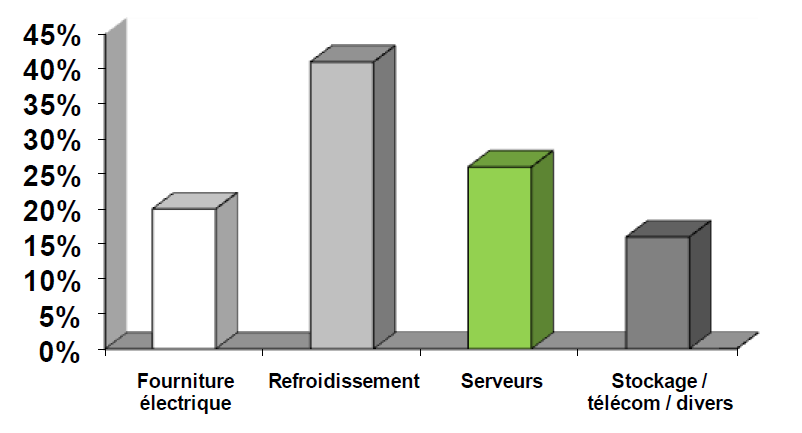
\includegraphics[scale=0.5]{figures/1.png} 
\end{center}
\caption{La consommation électrique dans les data centers}
\label{Cdatacenters}
\end{figure}

\section{Consommations d'énergie au niveau du systèmes de refroidissement}
\begin{onehalfspace}
Comme c'est illustrée dans la Figure 1.1, le refroidissement représente jusqu'à 50\% de la consommation d'énergie totale des data centers et des salles serveurs. Il est donc essentiel de concevoir un refroidissement efficace pour les sites informatiques quelle que soit leur taille.\medskip 

L'électricité consommée par les équipements informatiques est presque entièrement transformée en chaleur
par effet \textit{Joule}. Pour tenir à température constante le matériel, un système de refroidissement est nécessaire.
Sur un ordinateur personnel, ce rôle est tenu par un ou deux ventilateurs. Dans une salle contenant plusieurs
centaines d'équipements informatiques, l'installation d'une climatisation est nécessaire. Les nouveaux data centers déclarent souvent qu'ils utilisent des
sources froides naturelles, généralement de l'air, en complément de la climatisation.\medskip 

Il est possible de récupérer et de valoriser la chaleur produite par les climatisations. Cette chaleur pourrait
être valorisée dans des réseaux de chaleurs locaux dans une logique de filière énergétique locale. Pourtant,
la valorisation de la chaleur dans un réseau de chauffage urbain est rarement mise en œuvre lors de la
construction des data centers
\end{onehalfspace}

\section{Consommations d'énergie au niveau des serveur}
\begin{onehalfspace}
Les serveurs sont les équipements les plus énergétiques dans les data centers, ils consomment environ 40\% d’énergie totale des Data Centers. Ils constituent donc l’une des cibles prioritaires pour la mise en oeuvre des mesures d’économie d’énergie \cite{WEB47}.\medskip 

Pour traiter les données au sein de certains Data Centres, les serveurs n’utilisent que 6\% à 12\% d’énergie qu’ils consomment \cite{ref6}. Un serveur qui n’utilise que 20\% de sa capacité de calcul utilise déjà 70\% de sa puissance électrique maximale. Par ailleurs, une pièce jointe liée à un ancien mail de trois ans doit être stockée sur un serveur qui consomme de l’énergie pour fonctionner même si on  n’utilise plus la pièce jointe.\medskip 

24,7 milliards de dollars sont dépensés chaque année pour le matériel, la maintenance, la gestion, l’alimentation énergétique et le refroidissement des serveurs non utilisés. Cela représente environ le coût des 13 années du programme Apollo\footnote{Coûts du programme Apollo : 25,4 milliards de dollars.}\cite{ref8}.\medskip 

L’énergie consommée pour faire fonctionner ces serveurs non utilisés  compense les émissions du gaz CO$_{2}$ de 6,5 millions de véhicules.\medskip 

Un serveur à haute efficacité énergétique comporte des composants performants d’un point de vue énergétique, tels que les blocs d’alimentation, les processeurs, les disques durs, la mémoire et les connecteurs d’extension. À cette fin, des cartes mères pour serveur, plus efficaces que celles des générations précédentes sont également en cours de développement. L’idée générale est de minimiser les pertes liées à la transformation de courant sur la carte mère. Ces pertes sont  induites par l’écart entre la puissance d’entrée (sortie du bloc d’alimentation) et la puissance au niveau de chacun des composants \cite{WEB47}.


\begin{center}
\begin{tabular}{|c||c|}
\hline
\textbf{Composant} & \textbf{Puissance max (W)} \\
\hline
Processeur & 80 \\
\hline
Mémoire vive & 36 \\
\hline
Disques & 12 \\
\hline
Connecteurs d'extension & 50 \\
\hline
Carte mère & 25 \\
\hline
Ventilateurs & 10 \\
\hline
Alimentation & 38 \\
\hline
\end{tabular}
\captionof{table}{Exemples de puissance absorbée par différents composants}
\label{tab1}
\end{center}


Le tableau \ref{tab1} indique la consommation énergétique approximative de différents composants matériels et montre que les processeurs, les blocs d’alimentation, la mémoire vive et les bus de connecteurs d’extension sont ceux qui absorbent le plus de puissance.
\end{onehalfspace}

%\subsection{Efficacité du processeur}
%\begin{onehalfspace}

%\end{onehalfspace}

\section{Conclusion}
\begin{onehalfspace}
La problématique est donc la suivante : comment réduire la consommation d'énergie des serveurs sans pour autant trop impacter la qualité de service et les performances des applications qui s'exécutent sur le cloud ? Il existe de nombreux moyens pour réduire la facture d'électricité, et un bon nombre de techniques peuvent se faire sans impacter la qualité de service. Cependant, en acceptant une dégradation faible de performance, il est possible de réduire encore plus la puissance consommée par l'infrastructure.\medskip

Dans le prochain chapitre, nous allons présenté quelques techniques nécessaire pour réduire la consommation d'énergie dans les Data centers des Clouds.
\end{onehalfspace}


\chapter{Comment réduire l'impact énergétique des data centers ?}
\vspace{3cm}
\minitoc
\clearpage
\label{Chapitre2}
\section{Introduction}
\begin{onehalfspace}
%L'idée est de concentrer les traitements de données sur une machine et d'éteindre les autres. Il est ainsi possible d'éteindre des supports stockant des archives « mortes » etc. Les constructeurs proposent des solutions en ce sens (support pour les archives plus lent à réagir mais consommant moins d'énergie).\medskip \\
%Il s'agit d'une piste d'économie d'énergie qui ne nécessiterait que peu de modification physique dans un data center et qui mérite une attention particulière.\medskip \\
%La première question qu'il faut donc se poser est comment réduire la consommation d'énergie. Différents moyens sont à notre disposition, certains étant au niveau du fonctionnement de la machine elle même, et donc à une granularité de phases d'application, alors que d'autres sont à des niveaux plus hauts, et donc à une granularité d'application entière. Certains sont basés sur des leviers matériels, alors que d'autres sont purement applicatifs.\medskip \\
%Il est pourtant possible de gérer les serveurs et les opérations informatiques que doit effectuer un data center pour monter le taux d'utilisation à plus de 95\% [5].\medskip \\
%\lettrine[nindent=1em,lines=3]{A}fin d'agir sur la consommation d'énergie des data centers, nous possédons un ensemble de moyens bien différents. Ces moyens sont à différentes échelles, mais chacun a un impact sur cette consommation, et des effets souvent négatifs sur les performances. Ainsi, nous avons des leviers qui vont d'un niveau bas, au niveau processeur ou au niveau machine, à un plus haut niveau, de cluster ou d'infrastructure. Ces leviers peuvent être aussi bien logiciels, comme la virtualisation, que matériels, comme le DVFS.
%\subparagraph{}Nous essayerons dans cette partie de présenter les mécanismes actuellement disponibles et les principaux travaux de recherches qui ont été proposés.


\lettrine[nindent=1em,lines=3]{C}omme tout autre système distribué, les datas centers des clouds font face à une demande croissante en énergie. Cette énergie ne provoque pas seulement la diminution des bénéfices des fournisseurs mais aussi émette une grande quantité de dioxyde de carbone. Afin d’agir sur cette  consommation, les travaux de recherches dans la littérature présentent un  ensemble de techniques  bien différents pour résoudre ce problème. Ces moyens sont à différentes échelles mais chacun a un impact sur cette consommation et des effets souvent négatifs sur les performances du système. Ces techniques sont appliquées soit  à un niveau bas comme le processeur, soit à un niveau plus élevé de cluster ou d’infrastructure au niveau machine. Ces techniques peuvent être aussi bien logiciels comme la virtualisation que  matériels comme le DVFS (voir la section \ref{DVFS}).\medskip
\subparagraph{}Nous allons présenter dans ce chapitre quelques différentes techniques d’optimisations d’énergie et les principaux travaux de recherches qui ont été proposés dans la littérature.

\end{onehalfspace}
\section{Dynamic Voltage and Frequency Scaling}
\label{DVFS}
\begin{onehalfspace}
Le DVFS est un mécanisme mis en place par les constructeurs de puces. Il permet de réduire ou d’augmenter dynamiquement la fréquence d’un composant ainsi que son voltage. Cela permet de diminuer la fréquence d’un processeur lorsqu’il est sous utilisé, ou au contraire, d’augmenter sa fréquence au dessus de sa fréquence maximale  lorsqu’il a besoin d’être plus performant. Ce mécanisme se fait en réglant un couple de voltage/fréquence (appelés "Performance state" PState) dont les valeurs dépendront du processeur utilisé.\medskip

Les différents couples voltage/fréquence sont gérés par le système de la machine. C’est le cas dans les systèmes où sont implémentés des gestionnaires de fréquence CPU qu'on appelle gouverneur. Le but de ces gouverneurs  est de gérer la fréquence et le voltage du processeur en fonction d’une orientation définie par l’utilisateur et en fonction de certains paramètres systèmes. Trois gouverneurs différents sont implémentés par défaut : \textbf{performance}, \textbf{powersave} et \textbf{ondemand}. Le gouverneur \textbf{performance} réglera la fréquence au maximum, le \textbf{powersave} règlera la fréquence au minimum. Le gouverneur \textbf{ondemand} quand à lui règlera la fréquence au maximum dès l’arrivée des tâches à effectuer, il réduit  petit à petit cette fréquence quand la charge baisse.\medskip 

Néanmoins, toute action a un coût et le DVFS n’y échappe pas et peut ralentir une  application. Changer la fréquence prend du temps (de l’ordre de dizaine de microsecondes \cite{ref10}). Ce temps passe sans calcul. Par conséquent, des changements courants de fréquence vont avoir un impact très négatif sur les performances du système. Cet impact induira évidemment à un mauvais temps d’exécution de l’application (si cette application termine), ce qui donne une mauvaise consommation d’énergie. Il est important de noter qu’un autre inconvénient de la technique DVFS existe. Il peut arriver qu’une application consomme plus en tournant à une fréquence plus basse. Prenons par exemple une application qui se termine en 10 secondes avec un processeur qui consomme 100 W à une fréquence maximale. Nous aurons donc une consommation d’énergie de 1000 Joules. Admettons maintenant que cette même application consomme une fréquence minimale  de 50W mais prend  un temps de calcul de 30 secondes. Nous aurons alors une consommation d’énergie de l’application de 1500 Joules. Par contre, si cette application se termine en 15 secondes à fréquence minimale, nous aurons une consommation de 750 Joules.\medskip 

%Pour palier au problème de l'augmentation de la consommation d'énergie à basses fréquences, dans [43] les auteurs définissent un ordonnanceur visant à allouer les tâches HPC sous contrainte d'un budget d'énergie à ne pas dépasser. Ils utilisent les capacités apportées par le DVFS pour régler la fréquence des processeurs en fonction de l'échéance et du ralentissement prédits des tâches. Les résultats observé par simulation sur plus de 4000 processeurs montrent que les algorithmes que les auteurs ont défini apportent une augmentation de performance allant de 20\% à 40\% pour les tâches en comparaison avec une approche sans DVFS, tout en respectant la borne sur la consommation d'énergie.\medskip \\
Une vitesse d'exécution réduite n'implique pas forcément une réduction de la consommation d'énergie. Ce qui signifie que la réduction de la puissance n'implique pas non plus une réduction de la consommation d'énergie. Un bon exemple est décrit dans \cite{ref11}, où les auteurs présentent et implémentent un algorithme de scheduling basé sur des événements pour le gouverneur de processeur. Pour ce faire, les auteurs ont implémenté un scheduler qui reçoit des événements en fonction de la charge de travail. Ainsi, si la charge était basse au dessus d'un certain seuil, l'événement "chargé" va être envoyé et le gouverneur va ainsi changer la fréquence du processeur.\medskip 

La comparaison est faite notamment avec les gouverneurs implémentés dans les noyaux  Linux qui sont : performance (avec une fréquence maximale) et powersave (avec une  fréquence minimale). On remarque dans les résultats présentés par les auteurs que le gouverneur performance exécute le programme en 1h03 avec une puissance de 310W, cela  résulte une énergie de 329 Wh. On remarque aussi que le gouverneur powersave exécute ce même programme en 3h09 à une puissance de 284W résultant une énergie de 895Wh.  L’algorithme proposé dans cet article  exécute ce même programme en 1h05 avec une puissance moyenne de 298W avec  une énergie de 324Wh. Cela montre bien qu’il est nécessaire de bien utiliser  la gestion de fréquence des processeurs. Une fréquence plus faible n’économisera pas forcément de l’énergie et le bon choix sera parfois de favoriser la performance pour économiser l’énergie consommée avec un temps d’exécution plus court.\medskip 


Les auteurs dans \cite{ref12} tentent de résoudre  le  problème d’affectation de la fréquence la plus efficace en énergie en utilisant la charge de travail par intervalle. Cela est fait pour allouer la bonne fréquence et le bon voltage aux tâches. Ils ont proposé  un gouverneur visant à réduire la consommation d’énergie en minimisant les pertes de performance, acceptant ainsi des pertes pour avoir une  meilleure économie d’énergie. Pour cela, les auteurs caractérisent la charge de travail pour chaque nœud. Ils définissent ensuite le gouverneur efficace en énergie ecod basé sur les moments où le CPU attend le résultat d’activités hors processeur. Cela caractérise la charge en se basant sur des mesures sans avoir besoin d’aucune connaissance des applications qui s’exécutent sur le cluster. L’algorithme est ensuite évalué par l’exécution des benchmarks NAS Parallel Benchmark \cite{ref13}. Les auteurs montrent qu’une économie d’énergie allant jusqu’à 11\% peut être effectuée par rapport au gouverneur \textbf{ondemand} avec une faible perte de performance (5.1\% d’augmentation du temps de calcul contre 7.9\% pour \textbf{ondemand}).\medskip 


Un autre inconvénient de taille pour le DVFS est l'impact de la fréquence du DVFS sur le fonctionnement du processeur. En effet, des études montrent que l'utilisation du DVFS a un impact négatif sur la fiabilité du processeur \cite{ref14}. Les auteurs montrent analytiquement que réduire la fréquence à voltage fixe tend à réduire la performance (c'est-à-dire la probabilité de finir une application correctement avant échéance lorsqu'il y a des erreurs). De plus, réduire le voltage à des fréquences réduites augmente le taux d'erreurs dans les processeurs. \medskip 

L'approche de type DVFS n'est pas seulement limitée aux processeurs. C'est une approche qui peut être appliquée aussi à d'autres types de matériels. Par exemple, nous pouvons utiliser une approche similaire au niveau des cartes réseaux. Celle-ci s'appelle l'Adaptative Link Rate (ALR) \cite{ref15}. Le principe est le même : augmenter ou baisser la vitesse de la carte (son débit, faire fonctionner une carte Ethernet 1Gbps à 100Mbps ou moins) en fonction des besoins afin de limiter la consommation d'énergie. %Nous pouvons aussi effectuer le contrôle du voltage et de la fréquence au niveau des GPUs (Graphics Processing Unit), puisque ceux-ci sont utilisés dans certaines architectures hybrides CPU/GPU, où certains calculs sont effectués sur le GPU d'une machine, alors que les autres sont fait sur le CPU. Les GPUs sont de plus traditionnellement plus performants en terme de performance par watts pour les tâches très parallélisables, en en faisant des matériels intéressants pour améliorer l'efficacité énergétique des serveurs comme montré dans \cite{ref16}. Les auteurs dans \cite{ref16} montrent de plus qu'identifier les moments où il faut changer la fréquence et le voltage dans une architecture hybride CPU/GPU, permet d'atteindre des économies d'énergie de 28\% avec seulement une baisse de 1\% en performance dans le cas d'additions et de multiplications de matrices.\medskip 

%Ce genre d'approche est de plus en plus utilisée. Nous verrons de plus en plus de composants avec différentes vitesses possibles, et nous utiliserons de moins en moins explicitement ces capacités, car les fonctionnements seront directement intégrés, soit au niveau matériel, soit au niveau du système d'exploitation. Le but étant de s'approcher le plus possible d'infrastructures matérielles dites "proportionnelles", c'est-à-dire qui ne consomment qu'une énergie proportionnelle à leur charge.
\end{onehalfspace}

\section{Allumage et extinction des machines}
\begin{onehalfspace}

Il existe un moyen simple pour réduire la consommation d'énergie d’une machine. Il suffit de l’éteindre !
Par éteindre, nous entendons une extinction totale de la machine pour amener sa consommation à 0W. Cela est  possible par des appareils permettant de "désactiver" les prises de courant \cite{ref33}. Il faut bien faire la distinction entre une extinction et une mise en hibernation. Ce sont deux états similaires mais qui ne consomment pas la même puissance.
L’extinction de la machine désigne l’arrêt total de tous ses composants en réduisant la consommation de puissance à un niveau proche de 0W. Nous désignerons par  hibernation l’arrêt du système à l’exception de certains composants utilisés pour la mise en veille du système. Comme exemple d’hibernation, nous citons la carte réseau par l’utilisation du \textit{wake-on-lan} (technique consistant à réveiller une machine à distance par le réseau), le \textit{suspend-to-RAM} ou le \textit{suspend-to-Disk}.

La Figure \ref{EmachineLinux} est un exemple de diagramme des différents états d’une machine Linux. Elle présente les coûts en temps et en puissance électrique nécessaire pour passer d’un état à un autre. Les valeurs présentées sont tirées de \cite{ref17}.\medskip
\clearpage
\begin{figure}[!htb]
\begin{center}
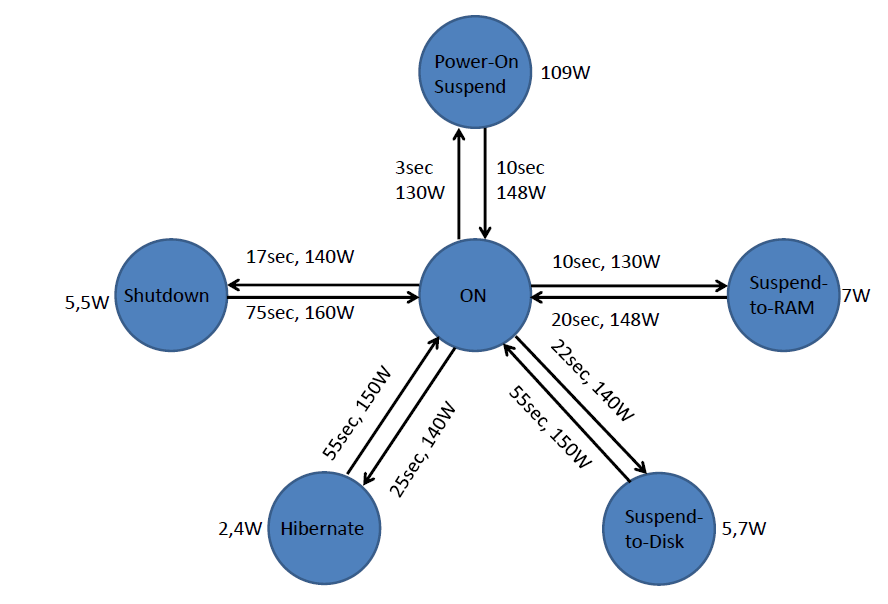
\includegraphics[scale=0.45]{figures/3.png} 
\end{center}
\caption{Exemple de transition entre états pour une machine Linux}
\label{EmachineLinux}
\end{figure}

Ainsi, il est possible de développer des approches utilisant cette technique afin de réduire
la consommation d'énergie. Dans \cite{ref18}, une approche utilisant un processus de décision de Markov est utilisée. Cette approche permet de  gérer les tâches,  l’état des hôtes (allumé ou éteint) et elle permet aussi d’atteindre l’état optimal pour la consommation d’énergie  tout en préservant la qualité de service (temps d’attente des tâches).\medskip

Cependant, pour réduire la consommation énergétique d'un serveur à 0W, nous devons prendre
en compte plusieurs facteurs.\medskip

Premièrement, nous devons être capables d’éteindre et de rallumer à distance les machines. Mais dans les clusters actuels, nous n’avons pas tout le temps cette capacité car les machines ne sont pas faites pour être éteintes. Deuxièmement, nous devons prendre en compte le temps pris pour éteindre et rallumer les différentes machines. Ce temps est équivalent au  temps pendant lequel les machines ne soient pas utilisées et consommeront de l’énergie. Il faut donc bien prendre en compte le temps d’allumage pour ne pas en avoir besoin en temps réel. Cela induit à une dégradation dans la qualité de service de la tâche. Enfin, il faut prendre en compte le coût induit par la consommation des ressources lors de l’allumage et l’extinction. C’est le cas lorsqu'on allume une machine. En plus du démarrage normal du système d’exploitation, cette machine  effectue une série de tests matériels et logiciels. Cela prend donc du temps mais aussi coûte de l’énergie dans la mesure où la machine fait des calcule. Ces temps et consommations d’énergie varient bien sûr en fonction de la machine, du système et des vérifications matérielles qui doivent être faites. Pour le temps d’allumage, cela peut aller jusqu’à la vingtaine de secondes dans \cite{ref19} à un peu plus d’une minute comme dans \cite{ref17}, voire même de plusieurs dizaines de minutes comme dans \cite{ref20}. \medskip


Toutefois, un effet indésirable peut apparaître lorsqu'on sollicite trop l'allumage et
l'extinction de matériels. Cela peut causer une augmentation du taux de malfonctionnement de
la machine. Bien que rien n'indique qu'au niveau machine le taux de malfonctionnement des hôtes ait
un lien avec le nombre de démarrage/extinction \cite{ref20}. Ce lien peut exister de la même manière  que pour le processeur et le DVFS comme c'est vu dans la section précédente \cite{ref14}.\medskip

L'allumage et l'extinction des hôtes physiques est donc une technique importante et extrêmement
puissante quand il s’agit de la réduction de  la consommation d’énergie d’un système informatique.
Ce moyen est  à utiliser avec précaution dans la mesure ou une mauvaise prédiction peut
causer des allumages/extinctions très fréquents  impliquant ainsi un gaspillage de ressources
et d’électricité. Il faut toujours que l'énergie économisée pendant qu'une machine reste éteinte soit plus
importante que celle consommée pendant l'allumage et l'extinction. C'est à dire augmenter la consommation d'énergie tout en dégradant la qualité de service.
\end{onehalfspace}

\section{Allocation}
\begin{onehalfspace}
L'allocation des tâches est aussi un moyen pour gérer la consommation d'énergie d'un système.
En plaçant de façon intelligente les tâches, nous pouvons utiliser les infrastructures les
moins gourmandes en électricité.\medskip

C’est le cas des techniques dites de consolidation. Le but étant de regrouper la charge de travail au même endroit pour pouvoir réduire la consommation d’énergie. Consolider les tâches sur un nombre réduit de machines peut avoir de graves effets. Outre le fait qu’on puisse tenter de consolider sans succès, il faut aussi prendre en compte les interactions que peuvent avoir les tâches entre elles lorsqu’elles s’exécutent sur une même machine. Dans \cite{ref21}, les auteurs montrent qu’en présentant la consommation de ressources d’une tâche, la consommation de ressources et l’énergie consommée par chaque transaction augmentent comparativement lorsqu’elle est seule. De plus, l’efficacité énergétique d’une transaction tend à augmenter aussi si la tâche s’exécute toute seule sur la machine. Les auteurs montrent ensuite qu’on peut trouver une zone optimale à laquelle chaque tâche s’exécutant sur la machine consommera le moins d’énergie. Ils proposent ensuite un algorithme de consolidation basé sur le profil des interactions des tâches pour déterminer la consolidation optimale ou proche de l’optimale, ainsi que pour caractériser quels types de charges de travail doivent être combinées.\medskip

L’allocation peut aussi être utilisée en tant que technique dans la mesure où une bonne caractérisation des différentes ressources matérielles peut faire une différence importante. Tous les serveurs ne consomment pas la même puissance pour exécuter la même application et donc l’utilisation de l’allocation des tâches s’avère donc importante. Différentes techniques peuvent être observées pour prendre en compte les différentes consommations à différents niveau, que ce soit au niveau du processeur ou au niveau de la machine elle-même.\medskip

C’est le cas par exemple de Dupont et al. dans \cite{ref22}, où les auteurs utilisent l’allocation et la réallocation des machines virtuelles pour mettre en oeuvre un framework flexible et efficace en énergie (ensemble de composants logiciels). Pour ce faire, les auteurs se basent sur  la gestion des clusters par la  programmation par contraintes sur Entropy \cite{ref23} afin d’être flexible en exprimant les différents objectifs pour les algorithmes. Cela donne la possibilité d’ajouter ou d’enlever des contraintes pour exprimer les contraintes SLA sans changer les algorithmes. Les auteurs valident ensuite leur framework par simulation et expérimentations. Ils montrent que dans un environnement cloud de test, leur approche permet de réduire jusqu’à 18\% d’émissions CO$_{2}$.

\end{onehalfspace}

\section{Virtualisation}
\begin{onehalfspace}
Au fur et à mesure que les systèmes deviennent de plus en plus complexes et les architectures de plus en plus diverses, il faut rendre transparent certains services. Il devient ainsi nécessaire d’avoir un accès commun à des ressources différentes pour faciliter le développement. C'est ici qu'intervient ce qu'on appelle la technique de  virtualisation. Cette technique permet de  rendre l’accès identique à plusieurs architectures. Par exemple, on peut avoir un accès virtualisé à des processeurs différents quel que soit leur constructeur ou leur méthode d’accès. La virtualisation peut être appliquée à plusieurs niveaux. Nous pouvons avoir la virtualisation du stockage où l'accès aux ressources de stockage sera transparent quel que soit l’endroit où se trouvent effectivement les disques durs et quel que soit  leur type (type normal, SSD, mémoire flash...) \cite{ref24}.\medskip 

Nous avons aussi  la virtualisation des machines virtuelles (VMs). Cela consiste à donner un accès complet à une infrastructure virtuelle qui apparait à l'utilisateur comme une machine complète (voir Figure \ref{Diagramme virtualisation avec un hyperviseur }). Cette technologie sert à donner à deux clients différents un accès chacun à une machine complète sur une même machine physique (PM). Cela permet d'avoir une meilleure sécurité dans le sens où même si on donne un accès administrateur à un utilisateur sur une machine virtuelle, ce dernier  ne pourra pas compromettre l'intégrité physique de la machine hébergeant la machine virtuelle \cite{ref25}. \medskip 
\clearpage
\begin{figure}[!h]
\begin{center}
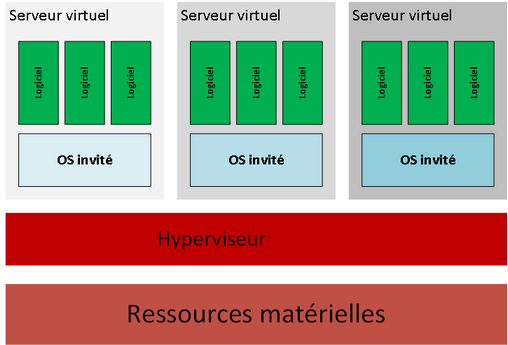
\includegraphics[scale=1]{figures/2.png} 
\end{center}
\caption{Diagramme virtualisation avec un hyperviseur }
\label{Diagramme virtualisation avec un hyperviseur }
\end{figure}


Les économies d'énergie réalisables grâce à la virtualisation sont de l'ordre de plus de 70\% à 80\%. Les économies réelles prélevées des projets de virtualisation dépendent du degré de virtualisation ainsi que du niveau de déploiement des nouvelles applications et fonctionnalités\cite{WEB26}.\medskip 

Les machines virtuelles ont l'avantage de permettre une séparation logique des ressources de la machine. Par exemple, on peut allouer deux machines virtuelles sur une même hôte en allouant par exemple 70\% du CPU à la première machine virtuelle et les 30\% restant à l'autre. Il apparaît donc que la gestion des tâches est facilitée par les technologies de virtualisation, notamment au niveau du pro-visionnement des tâches. Dans \cite{ref27}, les auteurs utilisent le fait que les machines virtuelles ne consomment pas tout ce qui leur est attribué pour sur-provisionner les machines physiques. Cela pour maximiser leur utilisation effective et économiser 20\% de ressources.\medskip 

La technique de virtualisation possède quelques inconvénients. Elle cause une baisse de performances. La gestion transparente des ressources est gérée par un intergiciel qui engendre des coûts de calculs et de gestion des ressources. Ainsi, un des inconvénients majeurs de la virtualisation est le surcoût associé à la virtualisation \cite{ref28}. Le surcoût est notamment dû au fait que d’une part l'accès aux ressources matérielles (GPU, disques durs, etc) est plus lent que l'intergiciel de virtualisation. Cet intergiciel  doit faire le lien entre le système hôte et la machine physique. Il est aussi dû au fait que les défauts de la page mémoire sont significativement plus coûteux. Ce surcoût dépend d'un certain nombre de paramètres tels que : le programme et l'architecture matérielle qui est virtualisée. Et peut atteindre des valeurs de ralentissement lorsque le cache est trop petit  (17\% pour une architecture Intel et 38\% pour une architecture AMD) \cite{ref28}.


\subparagraph{}La virtualisation offre une fonctionnalité nommée migration qui permet de migrer des machines virtuelles d'un nœud physique à un autre. Le but de cette technique est d'améliorer le temps de réponse et mieux gérer la consommation d'énergie.
\end{onehalfspace}

\section{Migration des machines virtuelles}
\begin{onehalfspace}
Les technologies actuelles de virtualisation permettent de migrer une machine virtuelle d'une machine physique à une autre. Cela peut se faire de deux manières. La première est une méthode qui consiste à mettre en pause la machine, la migrer et la reprendre une fois la migration terminée. La deuxième manière permet une migration dite à chaud. Il est possible de migrer une machine virtuelle presque sans perturber son fonctionnement, c'est-à-dire sans arrêter son fonctionnement mais avec une interruption de service minimale. Elle peut aller de 60ms pour un serveur de jeu à faible latence à 210ms pour un serveur avec un workload de type SPECweb99 \cite{WEB29}. Ce type de migration permet d'avoir une continuité du service avec juste une perturbation minimale au niveau réseau lors de la dernière partie de la migration \cite{ref30}.\medskip

Il existe plusieurs implémentations de la migration "live" de machines virtuelles. L'approche traditionnelle qui est implémentée dans Xen ou KVM par exemple est dite en pré-copie. Le processus de migration commence par une phase de pré-copie de la mémoire de
travail d'une machine virtuelle, puis va itérativement transférer à nouveau les pages qui ont
été utilisées par la machine virtuelle pendant le transfert précédent. Ceci jusqu'à l'obtention d'un
noyau de pages mémoire suffisamment petit ou jusqu'à ce qu'un nombre prédéfini d'itération
ait été effectué. La machine virtuelle est ensuite arrêtée et le noyau de mémoire final restant
à transférer est envoyé à la machine virtuelle destination qui est démarrée à son tour
marquant la fin de la migration.\medskip

Enfin, cette migration possède un coût non négligeable, qui entraîne une consommation de ressources sur l'hôte source et destination à la fois, ce qui augmentera la consommation d'énergie pendant la migration. De plus, les dernières phases de copie de la mémoire lors de la migration, juste avant de terminer celle-ci peuvent entraîner sur certaines machines une dégradation de la qualité de service. Par exemple, dans \cite{ref31}, les auteurs étudient le coût de la migration dans les clouds, avec des applications de type services web. Il apparaît que lors de la migration, le temps de réponse peut dans certains cas monter jusqu'à 3 secondes, induisant ainsi des violations de SLA\footnote{Le service level agreement (SLA) est un document qui définit la qualité de service requise entre un prestataire et un client.}.\medskip

Le coût de la migration peut être pris en compte dans la prise de décision afin de ne pas faire de ré-allocations de machines virtuelles et par conséquence ne pas perdre les  performances. C'est le cas de l'architecture de gestion de machines virtuelles de  GreenCloud proposé dans \cite{ref32}.

Il existe plusieurs techniques de migration des machines virtuelles, nous pouvons citer : la politique "Single Threshold" et la politique "Double Threshold".

\subsection{La politique "Single Threshold" (ST)}

La politique ST est basée sur l'idée de créer un seuil d'utilisation supérieur et de garder l'utilisation totale du CPU de toutes les machines physique en dessous de ce seuil.

\subsection{La politique "Double Threshold"}

L'idée est de fixer deux seuils, un seuil supérieur et un seuil inférieur et de garder l'utilisation totale du CPU de toutes les machines physiques entre ces seuils. L'objective de cette politique est de  réduire l'utilisation du processeur en dessous du seuil d'utilisation supérieur si le seuil supérieur est violé. Sinon si le seuil inférieur est violé, toutes les machines virtuelles doivent être migrées de cette machine physique et la machine physique doit être mise en état hors tension (etteinte). Nous allons définir maintenant les trois politiques basées sur la politique "Double Threshold".  

\subsubsection{La politique "Minimization of migrations" (MM)}

La politique MM sélectionne le nombre minimum de machines virtuelles nécessaires pour une migration.

\subsubsection{La politique "highest potential growth" (HPG)}

Lorsque le seuil supérieur est violée, HPG migre les machines virtuelles qui ont la plus faible utilisation de la CPU par rapport à la capacité de CPU définie par les paramètres des VMs. Cela pour minimiser l'augmentation potentielle de l'utilisation de l'hôte et et pour empêcher une violation SLA.

\subsubsection{La politique "The random choice" (RC)}

RC repose sur une sélection aléatoire d'un certain nombre de machines virtuelles nécessaire pour diminuer l'utilisation du processeur  en dessous d'un seuil d'utilisation supérieur.

\end{onehalfspace}
\clearpage
\section{Conclusion}
\begin{onehalfspace}
Dans ce chapitre, nous avons présenté quelques techniques d'optimisation d'énergie des data centers, en utilisant certains concepts tels que la virtualisation, la migration et la technique DVFS. Certaines techniques sont au niveau composant et d'autres sont au niveau infrastructure. Il convient donc de choisir les bonnes techniques pour arriver aux meilleurs résultats d'économies d'énergie et une bonne optimisation. Cela avec une perte minimale de performance et de qualité de service.

Le chapitre prochain consiste à implémenter une nouvelle stratégie de migration des machines virtuelles, Et cela dans le but d'améliorer certaines métriques de performance telle que la consommation d'énergie.
\end{onehalfspace}

\chapter{Conception}
\vspace{3cm}
\minitoc
\clearpage

\label{Chapitre3}


\section{Introduction}

\begin{onehalfspace}

\lettrine[nindent=1em,lines=3]{D}ans les chapitres précédents, nous avons exploré quelques techniques qui ont été proposées dans la littérature et qui ont un impact sur la consommation d'énergie.\medskip

Notre objectif principal est de proposer et d'implémenter une nouvelle stratégie de migration des machines virtuelles, Et cela dans le but d'améliorer certaines métriques de performance telle que la consommation d'énergie sans dégrader les contraintes du contrat SLA.\medskip

Le présent chapitre permet d'expliquer notre démarche en décrivant ses différentes phases, les algorithmes nécessaires pour son fonctionnement ainsi que les différentes étapes formalisées à l'aide du langage UML.
\end{onehalfspace}

\section{Approche proposée}
\begin{onehalfspace}
L’objectif de ce travail étant de proposer une stratégie basée sur la migration des machines virtuelles. Cette proposition permet de sélectionner le nombre minimum des machines virtuelles nécessaire à faire migrer à partir d’une machine physique.
L’avantage de cette stratégie est qu’elle permet d’augmenter considérablement le taux d’utilisation et de réduire la demande en énergie. L’idée de base est de concentrer les traitements de données sur une machine physique et d’éteindre les autres.

\end{onehalfspace}

\section{Architecture du système}
\begin{onehalfspace}
Dans cette partie, nous allons décrire le fonctionnement de notre modèle tout en formalisant et en utilisant une architecture qui sera la base de notre approche. Comme c’est illustrée dans la figure \ref{Architecture du système}, cette architecture est décrite par l’ensemble des composants suivants :
\clearpage
\begin{figure}[!h]
\begin{center}
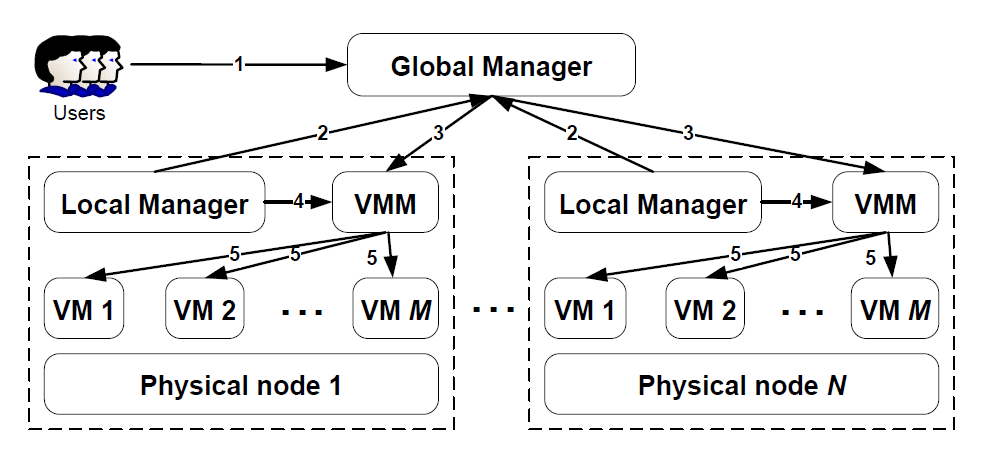
\includegraphics[scale=0.43]{figures/4.png} 
\end{center}
\caption{Architecture du système}
\label{Architecture du système}
\end{figure}
\begin{enumerate} [label=\Roman*)]
%\item \textbf{Data Center :} Un data center est une entité informatique composée d’un ensemble de machines physiques. Il est caractérisé par le nombre et la vitesse des processeurs, la capacité de la mémoire et de stockage, la bande passante ainsi que le coût de chaque ressource.
%\item \textbf{ Broker :} Le Broker assure la gestion des VMs dans plusieurs data centers et le routage du trafic vers les data centers appropriés. Il choisit aussi le data center qui fournit le meilleur  service pour les demandes envoyées par chaque utilisateur. Le Broker est responsable de la communication entre les utilisateurs et les data centers..
\item \textbf{Physical node :} Une machine physique est caractérisée par le nombre des VMs, la capacité, le nombre des requêtes arrivées, la vitesse du CPU et nombre de cores.
\item \textbf{VMs :}  Une machine virtuelle consiste à créer plusieurs environnements d'exécution sur une seule machine physique. Elle fournit à chaque utilisateur un service selon la demande.
\item \textbf{VM Manager (VMM):} Assure le suivi de la disponibilité des machines virtuelles et de leur utilisation des ressources. Il est chargé du provisionnement des nouvelles machines virtuelles ainsi que la réaffectation des VMs d’une machine physique à une autre afin d’adapter le placement.
\item \textbf{Local managers :} Les gestionnaires locaux se trouvent sur chaque noeud comme un module du VMM. Leur objectif est le suivi continu d’utilisation du processeur d’un noeud, le redimensionnement de la VM en fonction de leurs besoins en ressources et la prise de décision (quand et où les machines virtuelles doivent être migrées à partir d'un noeud physique).

\item \textbf{Global manager :} Il réside sur un nœud maître et recueille des informations auprès des gestionnaires locaux pour maintenir la vue globale de l'utilisation des ressources.
\end{enumerate}

Les gestionnaires locaux se trouvent sur chaque nœud en tant que module du moniteur de machine virtuelle (VMM). Leur objectif est le suivi continu d'utilisation du processeur d'un nœud, le redimensionnement de la VM en fonction de leurs besoins en ressources et la prise de décision (quand et où les machines virtuelles doivent être migrées à partir du nœud d'accueil) (4). Ils permettent aussi  de recevoir des requêtes à partir des clients (1). Le gestionnaire global réside sur un nœud maître et recueille des informations provenant des responsables locaux pour maintenir la vue d'ensemble de l'utilisation des ressources (2). Le gestionnaire global émet des commandes pour l'optimisation du placement VM (3). VMM effectue des redimensionnements réels et la migration des machines virtuelles ainsi que des changements dans les états d'alimentation des nœuds (5).
\end{onehalfspace}

\subsection{Calcul de la consommation d'énergie}
\begin{onehalfspace}

Ils existent plusieurs méthodes pour calculer la consommation d'énergie, parmi lesquels
nous avons utilisé la "méthode puissance par rapport à l'utilisation" : De nombreuses études, \cite{ref34}, \cite{ref35} ont montré que la consommation d'énergie par les serveurs peut être décrite par une relation linéaire entre la consommation d'énergie et l'utilisation du processeur. Ces études confirment qu'une puissance moyenne consommée par un serveur inactif est de 70\% de l'énergie consommée par rapport à un serveur pleinement utilisé et d'après \cite{ref36} , si l'utilisation du processeur est supérieure à 30\%, la valeur inférieure est toujours 0,3. Donc, ils ont défini la consommation d'énergie $P(u)$ par la Formule \ref{form1} :\bigskip

\begin{equation}
P(u) = Pmax \ast (0.7 + 0.3u)
\label{form1}
\end{equation}
\bigskip

\textbf{Tel que :}
$Pmax$ = 250w pour des serveurs modernes. La constante 0.7 est la puissance moyenne consommée par un serveur inactif quand le serveur est pleinement utilisé. \textit{u} : est l'utilisation du processeur. Comme l'utilisation de CPU peut changer avec le temps en raison de la variabilité de la charge de travail, il s'agit d'une fonction du temps: \textit{u(t)}. Par conséquent, pour définir la consommation d'énergie totale par un serveur, nous utilisons l'équation \ref{form3} \bigskip .\bigskip
\begin{equation}
E_{S} = \int_{t} {P(u(t)) dt}
\label{form3}
\end{equation}
\bigskip

Donc la consommation d'énergie par rapport à un data center est calculée par la Formule \ref{form2} \cite{ref37} : \bigskip

\begin{equation}
E_{D} = \frac{\sum_{j=1}^{m} P(u)_j}{m}
\label{form2}
\end{equation}
\bigskip

\textit{m} : nombre de machines physiques dans un data center.
\end{onehalfspace}
\subsection{Coût de la migration à Chaude des VMs}
\begin{onehalfspace}
La migration à chaude a un impact négatif sur les performances des applications en cours d'exécution dans une machine virtuelle pendant une migration. Voorsluys et al  \cite{ref38}, ont effectué une étude expérimentale pour étudier la valeur de cet impact et trouver un moyen de modélisation. Ils ont découvert que la dégradation des performances et des temps d'arrêt dépendent du comportement de l'application, c'est à dire, combien de pages mémoires sont mise à jour par l'application pendant son exécution. Pour les applications de web,  la dégradation de performance moyenne et  le temps d'arrêt peut être estimé à 10\% de l'utilisation du processeur. Cela signifie que chaque migration peut entraîner une certaine violation SLA. Il est donc essentiel de réduire au minimum le nombre de migrations de machines virtuelles. La durée d'une migration à chaude dépend de la quantité totale de mémoire utilisée par la machine virtuelle et la bande passante disponible. Pour nos expériences, nous définissons la dégradation des performances expérimentées par les $VM_j$ par la formule \ref{form4} \cite{ref43}: \bigskip

\begin{align}
 T_{m_{j}} = \frac{M_{j}}{B_{j}} \\
 U_{d_{j}} = 0.1\cdot \int_{t_{0}}^{t_{0}+T_{m_{j}}} {u_{j}(t) dt} \label{form4}
\end{align}
\bigskip

Où $U_{d_{j}}$ est la dégradation totale de performance par la $VM_j$, $t_{0}$ le temps où la migration commence, $T_{m_{j}}$ est le temps nécessaire pour terminer la migration, $u_{j}(t)$ est l'utilisation de la CPU par la $VM_j$, $M_{j}$ est la quantité de mémoire utilisée par la $VM_j$ et $B_{j}$ est la bande passante réseau disponible.
\end{onehalfspace}

\subsection{Violation de SLA}
\begin{onehalfspace}
Les exigences de la qualité de service sont extrêmement importantes pour le Cloud computing. Elles sont généralement formalisées sous forme de SLA\footnote{Service Level Agreement (SLA) est un document qui définit la qualité de service requise entre un prestataire et un client.}. Le contrat SLA peut être déterminé en termes de plusieurs contraintes  telles que le débit minimum ou le  temps de réponse maximum fourni par le système déployé. Etant donné que ces caractéristiques peuvent varier selon les applications, il est nécessaire de définir une métrique générique qui peut être utilisée dans notre simulation pour estimer le niveau du SLA qui est délivré par l’infrastructure. Pour ce qui nos concerne, nous définissons le niveau global de violation SLA causé par le système  comme une fraction de la différence entre les MIPS\footnote{MIPS : \textit{Million d'instructions par seconde}, unité de mesure des processeurs.} demandées par toutes les machines virtuelles $U_{r_{j}} (t)$ et les MIPS réellement alloués $U_{a_{j}} (t)$ . Cela est relatif au total des MIPS demandés au cours de la durée de vie des machines virtuelles ( voir équation \ref{form5}) \cite{ref43} . Où $M$ est le nombre de machines virtuelles.\medskip
\begin{align}
SLA = \dfrac{\sum_{j=1}^{M} \int_{t} U_{r_{j}} (t) - U_{a_{j}} (t) dt}{\sum_{j=1}^{M} \int_{t} U_{r_{j}} (t)}
\label{form5}
\end{align}\medskip

Cette métrique représente le pourcentage de la performance du CPU qui n'est pas afféctée lorsqu'elle est demandée par les applications relatives à la demande totale.
\end{onehalfspace}
\section{La stratégie de la minimisation des migrations des machines virtuelles}
\begin{onehalfspace}
Notre approche est divisée en deux phases: la sélection des VM à faire migrer  et l'allocation des VMs (voir Figure \ref{DiAMM}).

\begin{enumerate}
\item \textbf{Phase 1 : }Nous sélectionnons dans cette phase les machines virtuelles qui doivent être migrées (quelle VM doit-on choisir pour  faire une migration?) ;
\item \textbf{Phase 2 : }Les machines virtuelles choisies sont placées dans  les machines physiques à l’aide d’un algorithme de placement (quel  est le nouvel emplacement de la VM?).
\end{enumerate} 
\end{onehalfspace}
\clearpage
\begin{figure}[!h]
\begin{center}
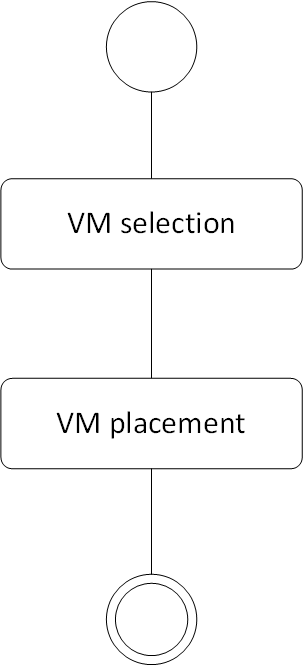
\includegraphics[scale=0.5]{figures/6.png} 
\end{center}
\caption{Diagramme d'activité de la migration des machines virtuelles}
\label{DiAMM}
\end{figure}



\subsection{Sélection des machines virtuelles}
\begin{onehalfspace}
Pour déterminer quand les machines virtuelles doivent être migrées, nous utilisons deux seuils d'utilisation du CPU (voir Figure \ref{DiASe}).
\subsubsection{Seuils d'utilisation fixe}
L’idée est de fixer deux seuils d’utilisation de CPU (seuil supérieur et seuil inférieur) et de garder l’utilisation totale du CPU de toutes les machines physique entre ces seuils. Si l’utilisation du CPU d’une machine physique est en dessous du seuil inférieur, toutes les VMs doivent être migrées de cette PM. Cette dernière est mise après en état hors tension (éteinte).

Si l’utilisation du CPU de la machine physique dépasse le seuil supérieur, on cherche la meilleure machine virtuelle pour faire une migration, afin de réduire l’utilisation de CPU. La meilleure VM est celle qui répond à deux conditions !
\begin{enumerate} [label=\Roman*)]
\item la machine virtuelle doit avoir une utilisation plus grande que la différence entre l’utilisation globale de CPU et le seuil supérieur.
\item la différence entre le seuil supérieur et la nouvelle utilisation de CPU est la plus petite. Si une telle VM n’existe pas, l’algorithme sélectionne la VM avec la plus grande utilisation CPU.
\end{enumerate}


\subsubsection{Seuils d'utilisation dynamique}
Comme mentionné précédemment, les seuils fixes ne sont pas adaptés pour un environnement avec des charges de travail dynamiques et imprévisibles. Cet environnement possède différents types d'applications qui peuvent partager la même ressource physique. Le système doit être capable d'ajuster automatiquement son comportement en fonction des modèles de charge de travail exposées par les applications. C'est pourquoi, nous utilisons une nouvelle technique pour calculer automatiquement les deux seuils d'utilisation CPU. Cette technique est basée sur sur une analyse statistique des données historiques recueillies au cours de la durée de vie des machines virtuelles \cite{ref44}. Nous allons présenter maintenant les formules permettant de calculer les seuils fixes.

\begin{enumerate}
\item \textbf{Seuil supérieur $T_{U_{i}}$:}
Nous avons calculé seuil supérieur $T_{U_{i}}$ comme montré dans \ref{tI}.
\begin{center}
\begin{equation}
U_{i} = \sum_{j=1}^{m} u_{j}
\end{equation}
\begin{equation}
S_{U_{i}} = \sqrt{\sum_{j=0}^{m} u_{j}^{2}}
\end{equation}
\begin{equation}
T_{U_{i}} = 1 - (((P_{uu} \ast S_{U_{i}}) + U_{i}) - ((P_{ul} \ast  S_{U_{i}}) + U_{i})
\label{tI}
\end{equation}
\end{center}
$u_{j}$ : L'utilisation du CPU de la machine virtuelle \textit{j}.\\
$m$ : Le nombre de machines virtuelles.\\
$U_{i}$ : L'utilisation du CPU de la machine physique \textit{i}.\\
$P_{uu}$ : égale à 95\% \cite{ref44}.\\
$P_{ul}$ : égale à 90\% \cite{ref44}.
\item \textbf{Seuil inférieur $T_{l}$:}
Nous avons calculé seuil inférieur $T_{l}$ comme montré dans 3.12.
\begin{center}
\begin{equation}
U_{i} = \frac{1}{m}\sum_{j=1}^{m} u_{j}
\end{equation}
\begin{equation}
S_{U_{i}} = \sqrt{(\sum_{j=0}^{m} u_{j} - U_{i})^{2}}
\end{equation}

\[
\label{TL}
T_{l} = \left\{
\begin{array}{r c l l l r}
U_{i} - (P_{l}*S_{U_{i}}) &,\textbf{Si}& L'utilisation& du& CPU < 0.3& (3.12)\\
0.3 &,\textbf{Si}& L'utilisation& du& CPU > 0.3
\end{array}
\right.
\]
\end{center}
$u_{j}$ : L'utilisation du CPU de la machine virtuelle \textit{j}.\\
$m$ : Le nombre de machines virtuelles.\\
$U_{i}$ : L'utilisation du CPU de la machine physique \textit{i}.\\
$P_{l}$ : égale à 90\% \cite{ref44}.
\end{enumerate}

\subsubsection{Phase de sélection des VMs}

La Figure \ref{DiASe} montre un diagramme d’activité qui résume la phase de sélection des machines virtuelles:
\clearpage
\begin{figure}[!h]
\begin{center}
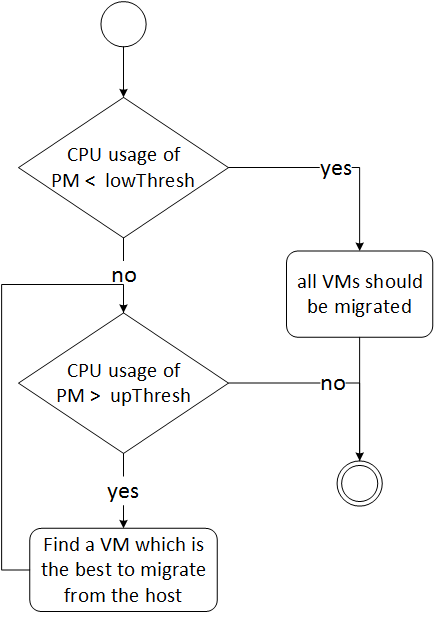
\includegraphics[scale=0.5]{figures/7.png} 
\end{center}
\caption{Diagramme d'activité de sélection des machines virtuelles}
\label{DiASe}
\end{figure}
L'algorithme \ref{ASe} illustre le pseudo-code de la procédure de sélection des machines virtuelles.
\clearpage
\RestyleAlgo{ruled}

\begin{algorithm}[!h]
%\DontPrintSemicolon
\SetAlgoVlined

\LinesNumbered
\Entree{hostList, vmList} \Sortie{migrationList}
\BlankLine
vmList.sortDecreasingUtilization()\;
\PourCh{h \textbf{dans} hostList}
{
	hUtil $\leftarrow$ h.util()\;
	bestFitUtil $\leftarrow$ MAX\;
	\Tq {hUtil $>$ h.upThresh()}
	{
		\PourCh{vm \textbf{dans} vmList}
		{
			\eSi{vm.util() > hUtil - h.upThresh()}
			{
				t $\leftarrow$ vm.util() - hUtil + h.upThresh()\;
				\uSi{t < bestFitUtil}
				{
					bestFitUtil $\leftarrow$ t\;
					bestFitVm $\leftarrow$ vm\;
				}
			}{
				\uSi{bestFitUtil = MAX}
				{
					bestFitVm $\leftarrow$ vm\;
				}\textbf{break}\;
			}
		}
		hUtil $\leftarrow$ hUtil - bestFitVm.util()\;
		migrationList.add(bestFitVm)\;
		vmList.remove(vm)\;
	}
	\Si{hUtil < h.lowThresh()}
	{
		migrationList.add(h.getVmList())\;
		vmList.remove(h.getVmList())\;
	}
}
\Retour{migrationList}\;
\caption{Algorithme de la sélection des machines virtuelles}
\label{ASe}
\end{algorithm}
L’algorithme \ref{ASe} est composé de deux parties :
La première partie de la ligne 5 jusqu’à la ligne 18 s’agit d’une boucle qui permet de réduire l'utilisation totale du CPU en dessous de seuil supérieur par sélection de quelques VMs à faire migrer. 
La seconde partie de la ligne 19 jusqu’à la ligne 21, il permet de vérifier si le seuil inférieur est violé, alors toutes les machines virtuelles seront migrées.   
\end{onehalfspace}
\subsection{Placement des machines virtuelles MBFD}
\begin{onehalfspace}
Pour déterminer l’emplacement des VMs migrées, nous utilisons l’algorithme MBFD\footnote{Modified Best Fit Decreasing (MBFD)}. Cet algorithme tri les  machines virtuelles dans l’ordre décroissant de leur utilisation de CPU. Il alloue  par la suite chaque VM dans une PM qui offre une consommation d’énergie minimale grâce à cette allocation (voir Figure \ref{DiAPl}).

La Figure \ref{DiAPl} montre un diagramme d’activité qui résume la phase de placement des machines virtuelles:

\begin{figure}[!h]
\begin{center}
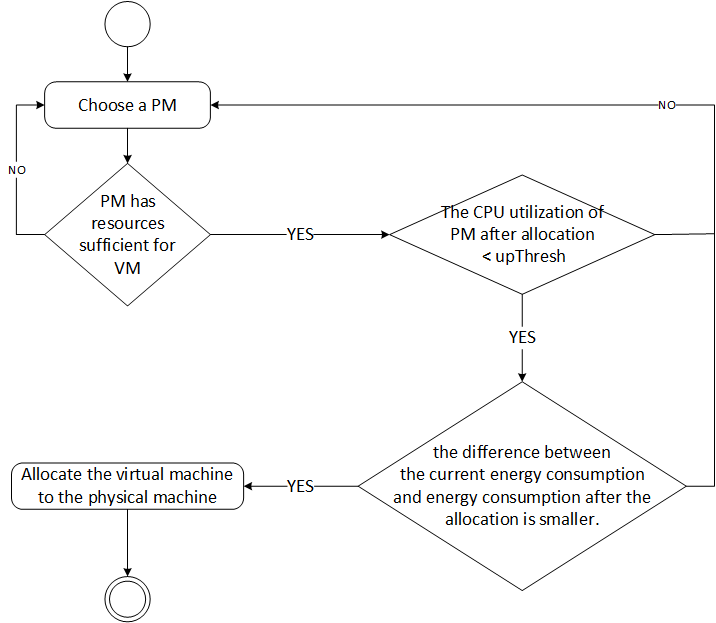
\includegraphics[scale=0.5]{figures/8.png} 
\end{center}
\caption{Diagramme d'activité de placement des machines virtuelles (MBFD)}
\label{DiAPl}
\end{figure}
\medskip
L'algorithme \ref{MBFD} illustre le pseudo-code de la procédure  de placement des machines virtuelles. 
\clearpage
\RestyleAlgo{ruled}

\begin{algorithm}[!h]
%\DontPrintSemicolon
\SetAlgoVlined

\LinesNumbered
\Entree{hostList, vmList} \Sortie{allocation of VMs}
\BlankLine
vmList.sortDecreasingUtilization()\;
\PourCh{vm \textbf{dans} vmList}
{
	minPower $\leftarrow$ MAX\;
	allocatedHost $\leftarrow$ NULL\;
	\PourCh{host \textbf{dans} hostList}
	{
		\Si{host a suffisamment de ressources pour vm}
		{
			power $\leftarrow$ estimatePower(host, vm)\;
			\Si{power < minPower}
			{
				allocatedHost $\leftarrow$ host\;
				minPower $\leftarrow$ power\;
			}	
		}
	}
	\Si{allocatedHost $\neq$ NULL}
	{
		allouer vm à allocatedHost\;
	}
}
\Retour{allocation}\;
\caption{Algorithme de placement des machines virtuelles (MBFD)}
\label{MBFD}
\end{algorithm}
L’algorithme \ref{MBFD} est composé de deux boucles imbriquées, la première boucle (ligne 2) permet de parcourir la liste des VMs à faire migrer. La seconde boucle (ligne 5) permet de parcourir la liste de toutes les PMs pour placer les VMs.

La complexité de l'algorithme \ref{MBFD} (MBFD) est $n*m$ , où \textit{n} est le nombre de noeuds et \textit{m} est le nombre des machines virtuelles qui doivent être migrées.
\end{onehalfspace}
\clearpage
\section{Conclusion}
\begin{onehalfspace}
Dans ce chapitre, nous avons présenté et décri les différentes étapes de notre stratégie proposée afin de minimiser le nombre de migration des machines virtuelles et par conséquence nous réduisant la consommation d’énergie .\medskip

Nous avons décrit le fonctionnement de notre proposition à l’aide d’un ensemble d'algorithmes, de formules et de diagrammes pour faciliter l'étude et la compréhension de notre proposition, d'une part, et pour donner un schéma général du travail demandé d'autre part.\medskip

En vue de concrétiser cette stratégie, nous allons décrire son implémentation dans le prochain chapitre sous le simulateur CloudSim, cela en utilisant le langage de programmation Java et l'environnement Netbeans.\medskip
\end{onehalfspace}

\chapter{Implémentation et Résultats}
\vspace{3cm}
\minitoc
\clearpage

\label{Chapitre4}

\section{Introduction}
\begin{onehalfspace}
\lettrine[nindent=1em,lines=3]{C}e chapitre est consacré à la réalisation et la concrétisation de nos approches proposées, qui consistent à minimiser l’énergie consommée  dans les  Cloud Computing. Il  aborde l’implémentation de notre stratégie. Nous allons commencer tout  d’abord par fixer l’environnement dans lequel nous avons réalisé notre simulateur. Nous allons définir par la suite  les métriques que nous avons utilisées. Enfin nous allons discuter  et analyser les résultats de la minimisation des migrations des machines virtuelles dans le Cloud Computing que nous avons obtenus.

\end{onehalfspace}
\section{Langage et environnement de développement}
\begin{onehalfspace}
L'environnement de développement est un facteur important qui doit être détaillé pour connaître dans quelles situations, le même travail peut être reproduit. La stratégie proposée dans le cadre de ce travail a été implémentée et testée dans l'environnement suivant :\medskip

\begin{itemize}
\item \textbf{Caractéristiques matérielles et logicielles du PC utilisé :} Nous avons développé notre application sur une machine avec un processeur Intel(R) Core(TM)i3-3110M CPU, une vitesse de 2.40Ghz et une capacité mémoire de 4GB. Le simulateur est  sous Windows 8.1 de 64bits.
\item \textbf{Simulateur utilisé :} CloudSim.
\item \textbf{Langage utilisé :} Java.
\item \textbf{IDE utilisé :} NetBeans.
\end{itemize}
\end{onehalfspace}
\subsection{Langage de programmation Java}
\begin{onehalfspace}
Java est à la fois un langage de programmation informatique orienté objet et un environnement
d’exécution portable. Il est céé par James Gosling et Patrick Naughton employés
de Sun Microsystems avec le soutien de Bill Joy (co-fondateur de Sun Microsystems en
1982), présenté officiellement le 23 mai 1995 au SunWorld \cite{ref39}.\medskip

Le langage Java a la particularité principale que les logiciels écrits avec ce dernier sont
très facilement portables sur plusieurs systèmes d’exploitation tels que : Unix, Microsoft
Windows, Mac OS ou Linux avec ou sans modifications. C’est la plate-forme qui
garantit la portabilité des applications développées en Java \cite{ref39}.\medskip

Les applications Java peuvent être exécutées sur tous les systèmes d’exploitation pour
lesquels a été développée une plate-forme Java dont le nom technique est JRE (Java Runtime
Environment - Environnement d’exécution Java). Cette dernière est constituée d’une
JVM (Java Virtual Machine - Machine Virtuelle Java), le programme qui interprète le code
Java et le convertit en code natif. Mais le JRE est surtout constitué d’une bibliothèque
standard à partir de laquelle doivent être développés tous les programmes en Java. C’est
la garantie de portabilité qui a fait la réussite de Java dans les architectures client-serveur
en facilitant la migration entre serveurs, ce qui est très difficile pour les gros systèmes \cite{ref40}.\medskip

Java est devenu aujourd’hui une direction incontournable dans le monde de la programmation
parmi les différentes caractéristiques qui sont attribuées à son succès , nous avons \cite{ref39} :\medskip

\begin{itemize}
\item L’indépendance de toute plate-forme : le code reste indépendant de la machine sur
laquelle il s’exécute. Il est possible d’exécuter des programmes Java sur tous les
environnements qui possèdent une Java Virtual Machine.
\item Java est également portable, permettant à la simulation d’être distribuée facilement
sans avoir à recompiler le code pour les différents systèmes.
\item Le code est structuré dans plusieurs classes dont chacune traite une partie différente
de la simulation.
\item Il assure la gestion dynamique de la mémoire.
\item Java est multitâches : il permet l’utilisation de Threads qui sont des unités d’exécution
isolées.

\end{itemize}

Aussi, une des principales raisons de ce choix est que le simulateur CloudSim est développé
avec ce langage.

\end{onehalfspace}

\subsection{Environnements de développement}
\begin{onehalfspace}
NetBeans est un environnement de développement intégré (EDI), placé en Open Source par Sun en Juin 2000. En plus de Java, NetBeans permet également de supporter différents autres langages, comme Python, C, C + +, JavaScript, XML, Ruby, PHP et HTML téléchargeable du site : \url{https ://netbeans.org/downloads}. Il comprend toutes les caractéristiques d’un IDE moderne (éditeur en couleur, projets multi-langage, refactoring, éditeur graphique d’interfaces et de pages Web).\medskip

Conçu en Java, NetBeans est disponible sous Windows, Linux, Solaris, MacOSX ou sous une version indépendante des systèmes d’exploitation (requérant une machine virtuelle Java).\medskip

De plus, NetBeans est écrit en Open Source, téléchargeable directement du site \url{http ://java.sun.com}. Il est puissant et compatible avec toutes les nouvelles technologies Java (les technologies Java EE, les bases de données, UML, XML, ...).
\end{onehalfspace}

\subsection{Simulateur CloudSim}
\begin{onehalfspace}
CloudSim est une nouvelle structure de simulation généralisée et extensible qui permet
la modélisation des environnements hétérogènes, la simulation et l’expérimentation de
Cloud émergent des infrastructures de calcul et des services d’application. Il offre les
fonctionnalités suivantes :\medskip
\begin{itemize}
\item Une plate-forme indépendante pour la modélisation des Data Centers, des Brokers, de l'ordonnancement et des politiques d'allocation des ressources;
\item Support pour la modélisation et la simulation à grande échelle d’infrastructure de
Cloud Computing, y compris des centres de données sur un seul noeud physiques.
\end{itemize}\medskip

Parmi les principales caractéristiques de CloudSim, nous pouvons citer :
\begin{itemize}
\item La flexibilité pour commuter entre l’allocation en espace et en temps
partagé 
et la prise en charge de la répartition des coeurs de traitement aux services
virtualisés;
\item La disponibilité d’un moteur de virtualisation qui facilite la création et la gestion
indépendante des services ainsi que l’hébergement des services virtualisés sur un
noeud d’un Datacenter ;
\item Un support pour la simulation des connexions réseau entre les éléments du système
de simulation ;
\item Simulation de la définition de matériel de centre de traitement des données (Datacenter)
en termes de machines physiques composées de processeurs, de dispositifs
de stockage, de mémoire et de largeur de bande interne ;
\item Simulation des spécifications, de la création et de la destruction de machines virtuelles
;
\item Simulation de l’exécution des programmes utilisateurs ou des demandes (Cloudlet)
sur les machines virtuelles.

\end{itemize}
Nous avons utilisé pour la réalisation de notre travail la version du simulateur CloudSim 2.1.1 téléchargeable du site : \url{https ://code.google.com/p/cloudsim/downloads/list}.
\end{onehalfspace}
\subsubsection{Architecture de CloudSim}
\begin{onehalfspace}
La structure logicielle de CloudSim et ses composants sont représentés par une architecture en couches comme c'est montré dans la Figure \ref{Architecture du système}. Les premières versions de CloudSim utilise SimJava, un moteur de simulation d'événement discret qui met en oeuvre les principales fonctionnalités requises pour des structures de simulation de haut niveau. Parmi les fonctionnalités, nous avons la formation d'une file d'attente et le traitement d'événements, la création de composants système (les services, les machines (Host), le centre de données (Datacenter), le courtier (Broker), les machines virtuelles), la communication entre les composants et la gestion de l'horloge de simulation :

\begin{figure}[!h]
\begin{center}
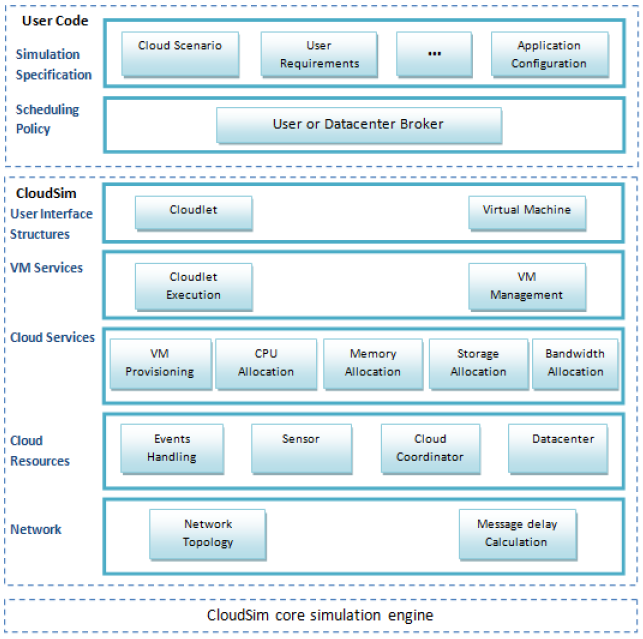
\includegraphics[scale=0.5]{figures/5.png} 
\end{center}
\caption{Architecture de CloudSim \cite{ref41}}
\label{ArchitecturedeCloudSim}
\end{figure}

\end{onehalfspace}

\subsubsection{Classes de CloudSim}

\begin{onehalfspace}
Le simulateur CloudSim est composé de plusieurs classes que nous pouvons classer en deux catégories : des classes qui modélisent les entités comme le Data Center, le Broker, etc. Et des classes modélisant les politiques d'allocation.

Parmi les classes fondamentales qui forment les blocs constitutifs du simulateur CloudSim comme est présenté dans la Figure \ref{ClassCloudSim} , nous pouvons citer seulement celles utilisées :
\begin{figure}[!h]
\begin{center}
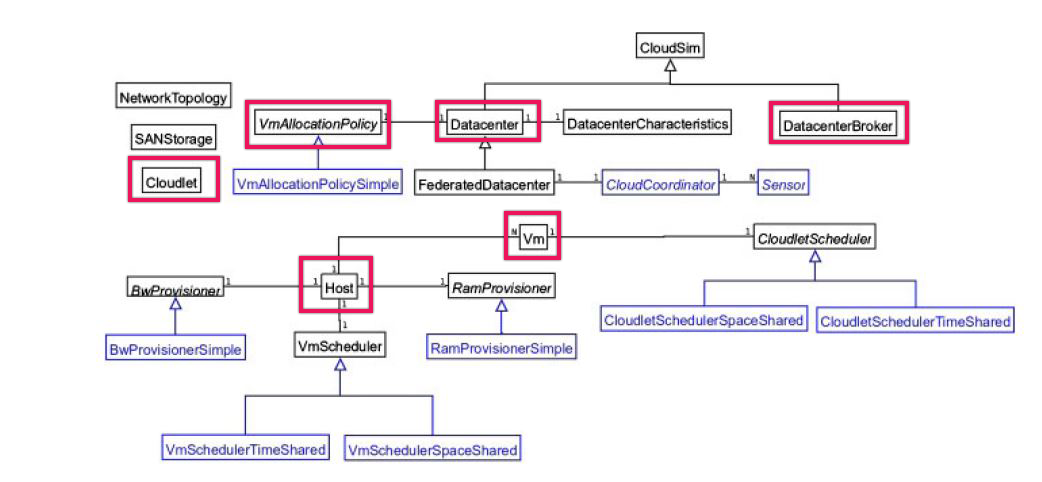
\includegraphics[scale=0.52]{figures/cloudsimclass.png} 
\end{center}
\caption{Diagramme de classe de la conception de simulateur CloudSim}
\label{ClassCloudSim}
\end{figure}
 
\begin{enumerate} [label=\Alph*.      ]
\item \textbf{Cloudlet :} Cette classe modélise les services d'application du Cloud (comme la livraison, réseaux
sociaux, et le workflow d'affaires). CloudSim représente la complexité d'une application en fonction de ses besoins informatiques. Chaque service d'application a une taille d'instruction pré-assigne et la quantité de flux de transfert de données qu'il doit entreprendre au cours de son cycle de vie. Cette classe peut également être étendu pour supporter la modélisation de la performance et d’autres paramètres de composition pour les applications telles que les transactions dans les applications orientées base de données \cite{ref45}.
\item \textbf{Datacenter :} Cette classe modélise les services au niveau des infrastructures de base (matériel) qui sont offerts par les fournisseurs de Cloud (Amazon, Azure, App Engine). Elle encapsule un ensemble de hôtes qui peuvent être soit homogènes ou hétérogènes par rapport à leurs configurations matérielles (mémoire, noyaux, capacité et stockage) \cite{ref45}.
\item \textbf{DatacenterBroker :} Cette classe modélise le Broker, qui est responsable de la médiation entre les utilisateurs et les prestataires de service selon les conditions de QoS des utilisateurs et il déploie les tâches de service à travers les Clouds. Le Boker au nom des utilisateurs, agit sur les prestataires du service approprié du cloud par le service d’information du Cloud CIS (Cloud Information Services) et négocie avec eux pour une allocation des ressources qui répond aux besoins de QoS des utilisateurs. Les chercheurs et développeurs des systèmes doivent étendre cette classe pour évaluer et tester les politiques de courtage personnalisées. \cite{ref45}.
\item \textbf{DatacenterCharacteristics :} Cette classe contient les informations sur la configuration des ressources des centres de données \cite{ref45}. 
\item \textbf{Host :} Cette classe modélise une ressource physique comme le serveur de stockage ou de calcul. Elle encapsule des informations importantes telles que la quantité de mémoire et de stockage, le type de coeurs de traitement (pour représenter une machine multi-core), une politique d’allocation pour le partage de la puissance du traitement entre les machines virtuelles et les politiques d’approvisionnement de mémoire et de bande passante pour les machines virtuelles \cite{ref45}.
\item \textbf{SimEntity :} Il s'agit d'une classe abstraite, elle représente l’entité de simulation qui est capable d'envoyer des messages à d'autres entités et de gérer les messages reçues ainsi que les événements. Toutes les entités doivent étendre cette classe et redéfinir ses trois principales méthodes : \textit{startEntity()}, \textit{processEvent()} et \textit{shutdownEntity()}. Ces méthodes définissent les actions pour l'initialisation de l’entité, le traitement des événements et la destruction de l’entité \cite{ref45}.
\item \textbf{VM :} Cette classe représente une instance de machine virtuelle (VM) qui est gérée et hébergée par une machine physique (hôte). Chaque composant VM a accès à un composant qui stocke les caractéristiques suivantes liées à une VM telles que: mémoire accessible, le processeur, capacité de stockage, et les politiques de provisionnement interne de la machine virtuelle qui est étendu à partir d'un composant abstrait appelé le CloudletScheduler \cite{ref45}.
\item \textbf{VMAllocationPolicy :} C'est une classe abstraite implémentée par un composant hôte qui modélise les politiques (d'espace partagé, de temps partagé) exigées pour allouer la puissance de traitement aux VMs. Les fonctionnalités de cette classe peuvent facilement être ignorées pour accommoder des politiques spécifiques à l'application de partage de processeur \cite{ref45}.
\item \textbf{VMProvisioner :} Cette classe abstraite représente la politique d'approvisionnement qu'un moniteur de VM utilisé pour allouer les VMs aux hôtes. La VMProvisioner sélectionne l’hôte qui répond à la quantité de mémoire demandée, le stockage pour le déploiement de la VM \cite{ref45}.
\end{enumerate} 
\end{onehalfspace}


\section{Description du fonctionnement de notre logiciel}
\begin{onehalfspace}
Nous présentons dans cette partie une vue globale de notre simulateur en détaillant les différentes étapes à effectuer pour réaliser une simulation.

Selon le diagramme de la Figure \ref{DiAFL}, la simulation commence après :

\begin{enumerate}
\item \textbf{Création du Cloud : } étape permettant de créer l’architecture Cloud en spécifiant le nombre de DataCenters.
\item \textbf{Configuration de Data Center : } Cette étape permet de spécifier les caractéristiques du Data Center telle que le nombre de nœuds physiques, la bande passante, etc.
\item  \textbf{Configuration des PMs : } Cette étape permet de créer une machine physique et spécifier ses caractéristique telle que nombre de processeurs, la capacité de stockage, etc.
\item  \textbf{Configuration des VMs : } Cette étape permet de créer une machine virtuelle.
\end{enumerate}
\begin{figure}[!h]
\begin{center}
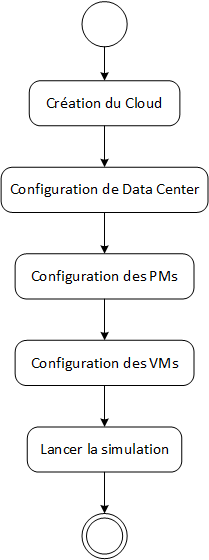
\includegraphics[scale=0.95]{figures/9.png} 
\end{center}
\caption{Diagramme d’activité du fonctionnement de notre logiciel}
\label{DiAFL}
\end{figure}
\end{onehalfspace}
\section{Implémentation}
\begin{onehalfspace}
Dans cette partie, nous allons nous intéresser à la démonstration de notre application à travers un exemple en faisant référence à quelques interfaces graphiques.
\subsection{Accès à l’interface}
La version de CloudSim n’a pas d’interface graphique, son exécution se fait sur la console donc nous avons créé une interface qui facilite l’accès au simulateur. L’interface doit faire appel à CloudSim ainsi qu’aux différentes approches qui se trouvent dans différents packages.\medskip

La Figure \ref{InterfacePrincipale} représente la première interface de notre simulateur qui apparaît à l'utilisateur. 

\begin{figure}[!h]
\begin{center}
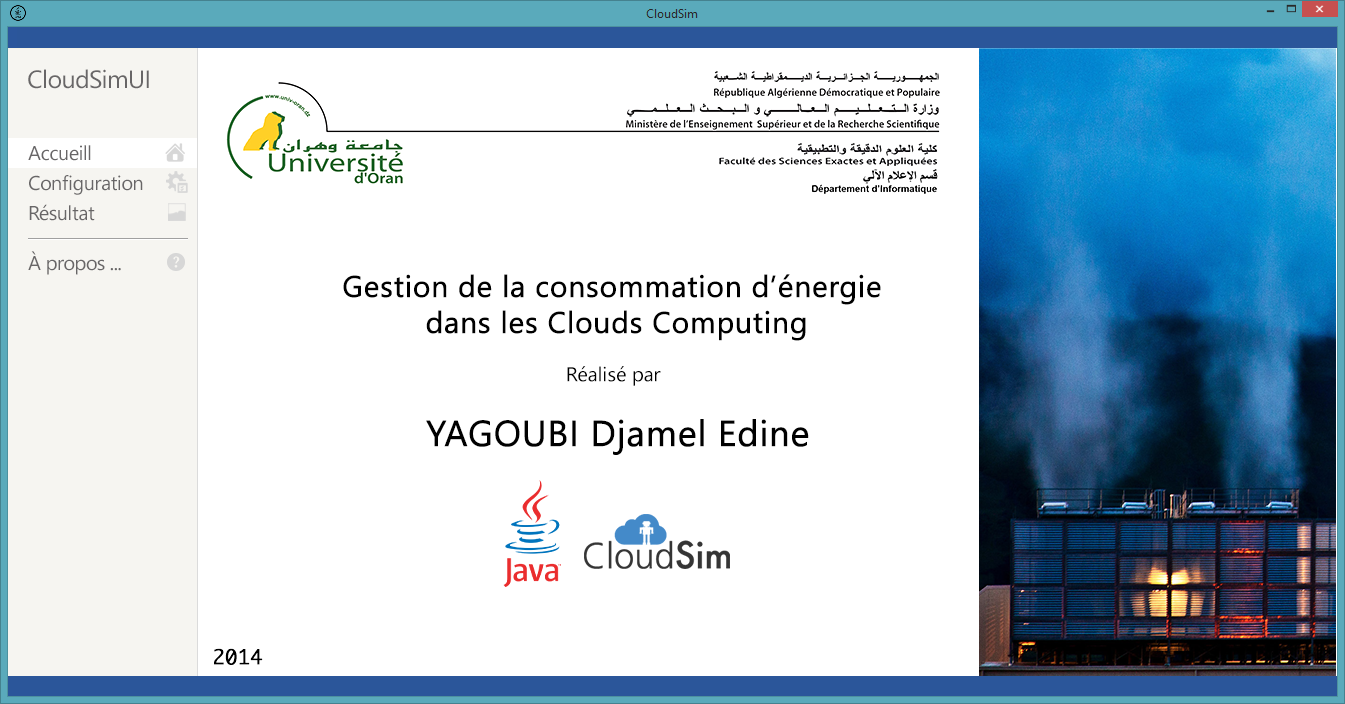
\includegraphics[scale=0.4]{figures/inf1.png} 
\end{center}
\caption{Interface principale}
\label{InterfacePrincipale}
\end{figure}

\subsection{Configuration de Simulation}
La première action à effectuer est la configuration des composants du Cloud. Cette configuration est réalisée en quatre étapes :
\subsubsection{Configuration du Data Center}

Cette étape consiste à faire entrer les caractéristiques du Data Center (voir Figure \ref{ConfigurationdeDatacenter} ) comme : le nom du Data Center, l'architecture de système d'exploitation, le coût de traitement, le coût de la mémoire, le coût de stockage, le coût de la bande passante , l'intervalle de l'ordonnancement et le système d'exploitation. 

\begin{figure}[!h]
\begin{center}
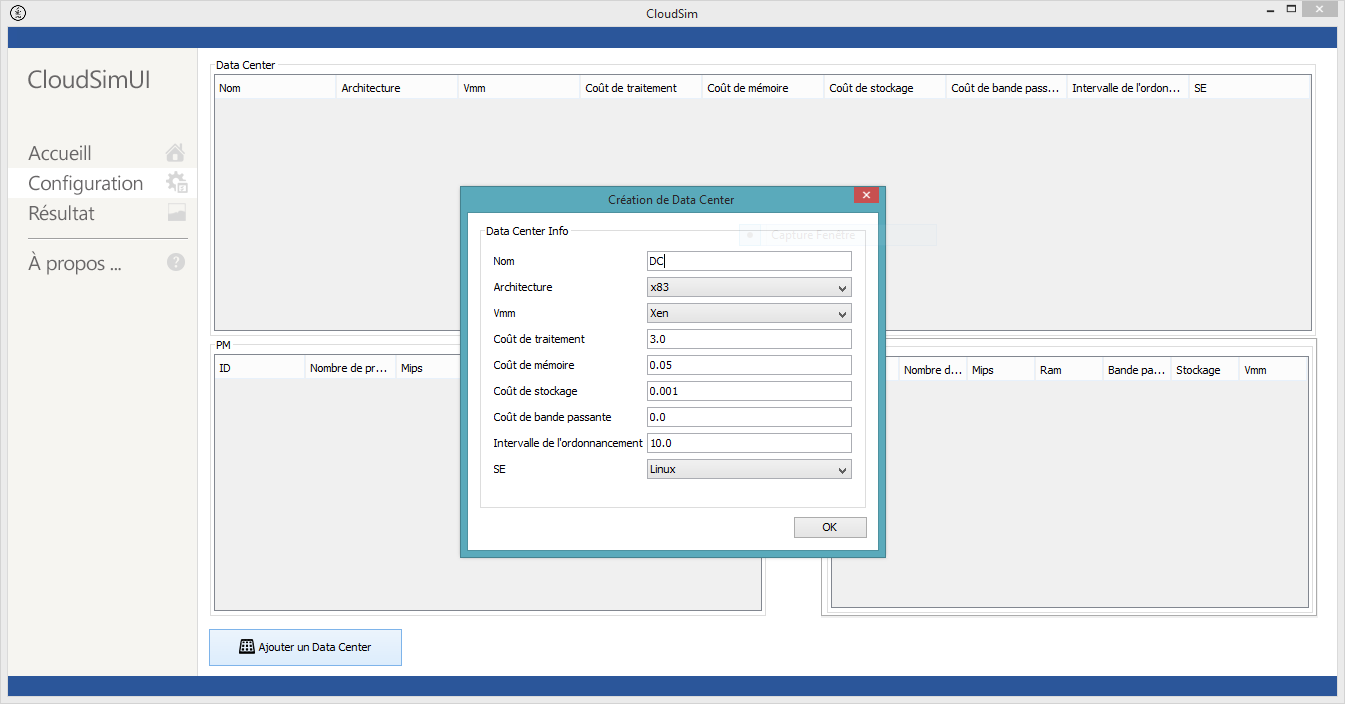
\includegraphics[scale=0.4]{figures/inf2.png} 
\end{center}
\caption{Configuration du Data Center}
\label{ConfigurationdeDatacenter}
\end{figure}
\subsubsection{Configuration des machines physiques}
La Figure \ref{Configurationdesmachinesphysiques} représente l’étape de création des machines physiques. Le bouton \textit{\textbf{Ajouter des machines physiques}} permet de créer des machines physiques hétérogènes en précisant le nombre des hôtes, nombre de processeur, MIPS, RAM, capacité de stockage et la bande passante.
\clearpage
\begin{figure}[!h]
\begin{center}
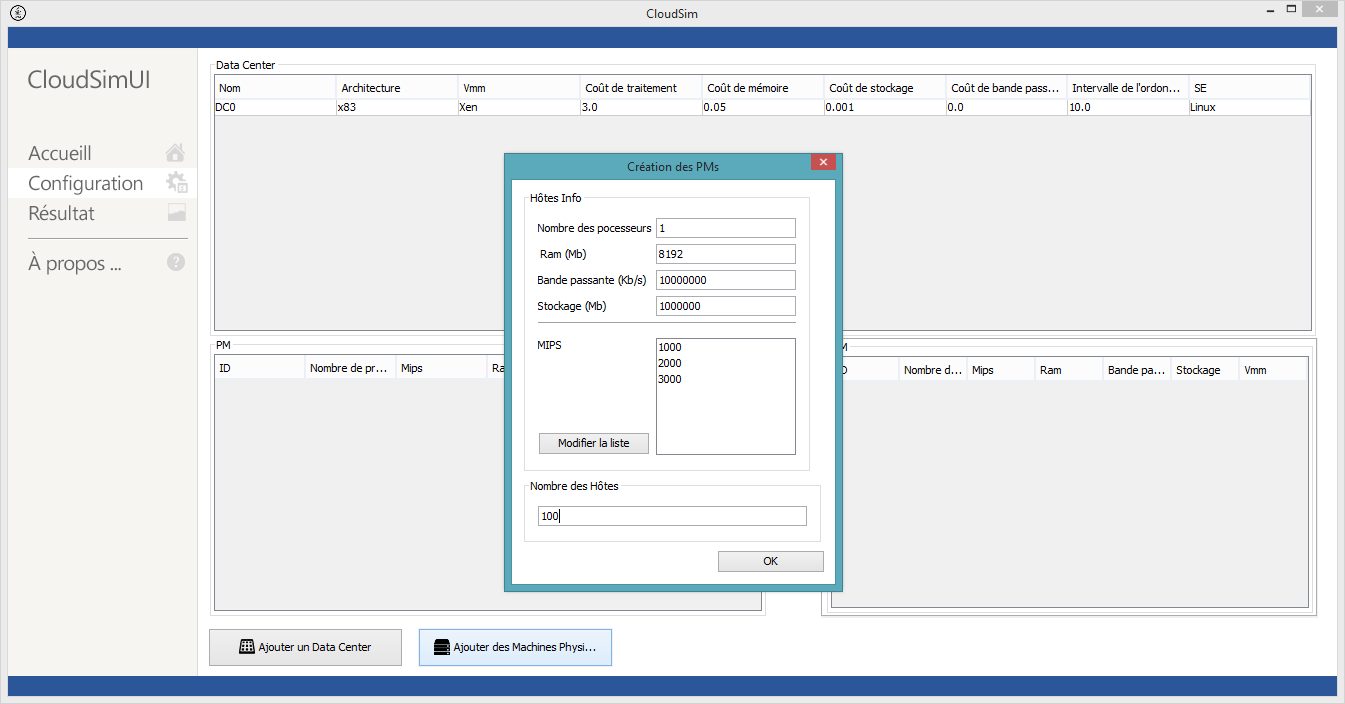
\includegraphics[scale=0.4]{figures/inf3.png} 
\end{center}
\caption{Configuration des machines physiques}
\label{Configurationdesmachinesphysiques}
\end{figure}

\subsubsection{Configuration des machines virtuelles et Cloudlets}

La création des Cloudlets et des machines virtuelles hétérogènes  se fait en cliquant sur le bouton \textbf{Ajouter des machines virtuelles} (voir Figure \ref{CMVCs}). Pour cela, il faut  préciser le nombre des Cloudlets, le nombre de processeur, MIPS, RAM, capacité de stockage, la bande passante, taille de cloudlet, taille de fiché de cloudlet et la  taille de sortie de cloudlet.

\clearpage
\begin{figure}[!h]
\begin{center}
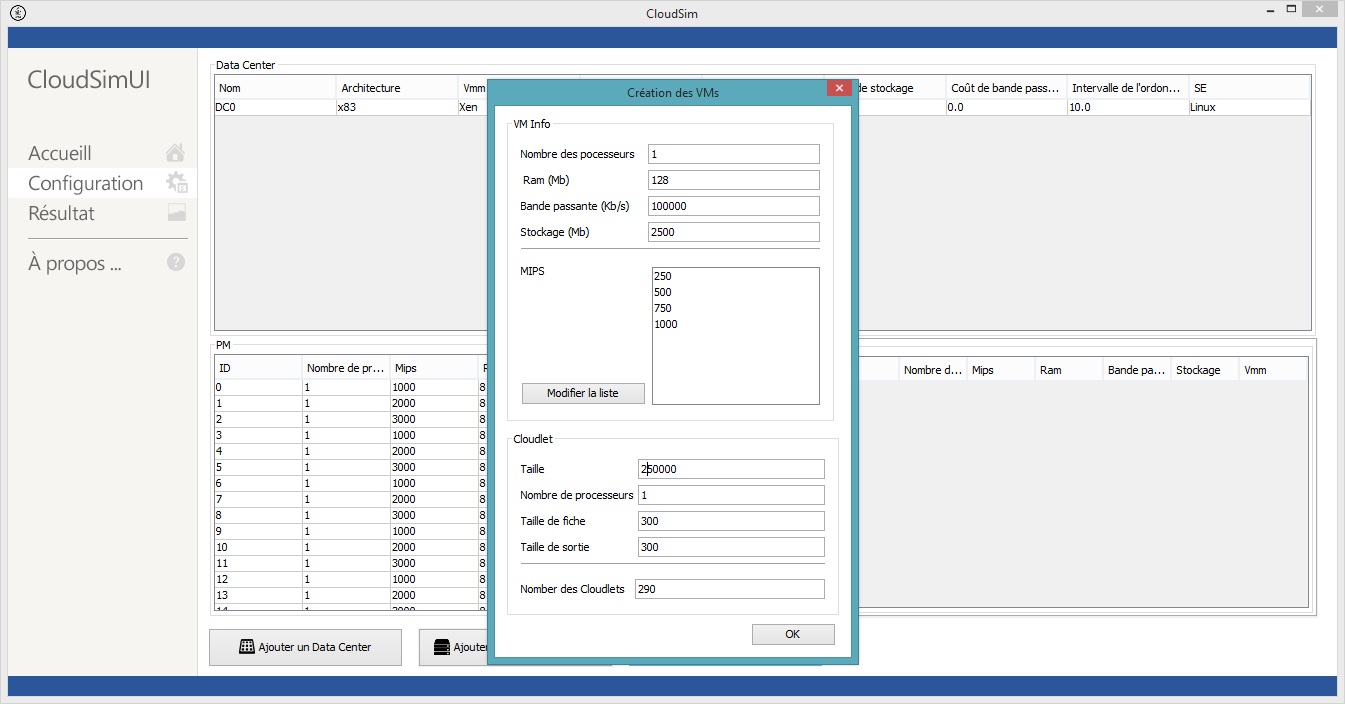
\includegraphics[scale=0.4]{figures/inf4.png} 
\end{center}
\caption{Configuration des machines virtuelles et Cloudlets}
\label{CMVCs}
\end{figure}

\subsubsection{Lancement de la simulation}
Le bouton \textit{\textbf{Lancer la simulation}} illustré dans la Figure \ref{LDS} permet de choisir les paramètres de simulation en spécifiant le nombre de simulations, le seuil de l'approche \textit{ \textbf{Single Threshold }} et les seuils supérieurs et inférieurs de l'approche  \textit{\textbf{Fixed Double Threshold}}. Nous pouvons lancer les simulations en cliquant sur le bouton \textit{\textbf{OK}}. 
\clearpage
\begin{figure}[!h]
\begin{center}
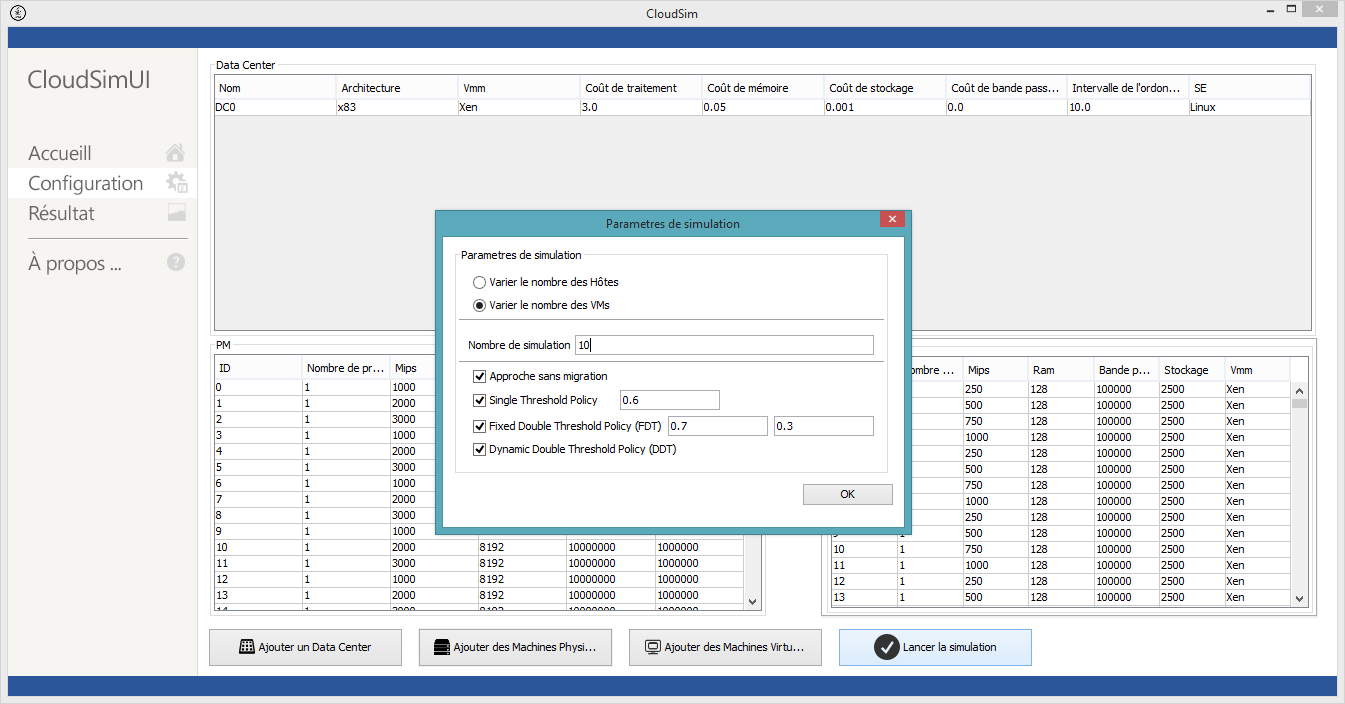
\includegraphics[scale=0.4]{figures/inf5.png} 
\end{center}
\caption{Lancement de la simulation}
\label{LDS}
\end{figure}

\subsubsection{Résultat}
Le bouton « Résultat » permet à son tour d’afficher les résultats des simulations représentées dans le graphe (voir Figure \ref{Résultat}) à l’aide d’un API java JFreeChart\footnote{\textbf{JFreeChart} est une API Java permettant de créer des graphiques et des diagrammes de très bonne qualité.}.
\clearpage
\begin{figure}[!h]
\begin{center}
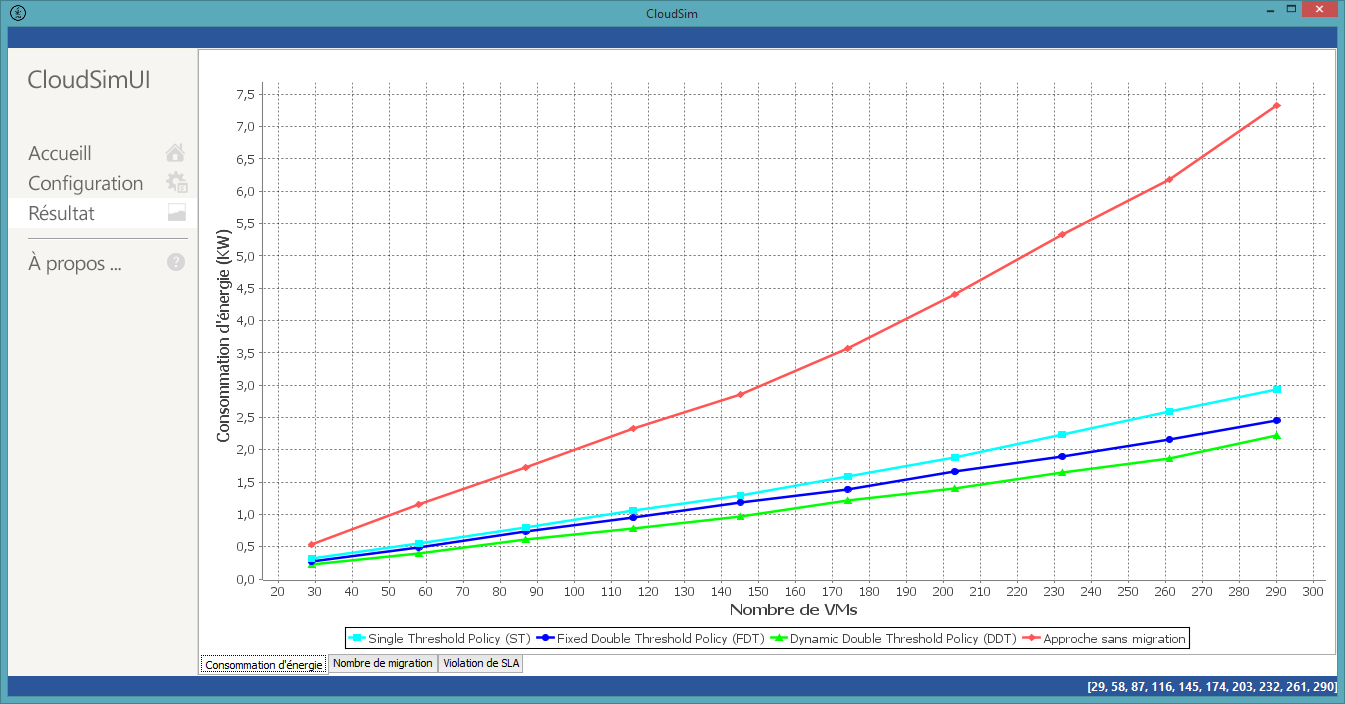
\includegraphics[scale=0.4]{figures/inf6.png} 
\end{center}
\caption{Résultat}
\label{Résultat}
\end{figure}

\end{onehalfspace}

\section{Expérimentations}

\begin{onehalfspace}
Pour mettre en valeur les apports de nos approches, nous allons se focaliser sur les métriques suivantes : l’énergie consommée, nombre de migrations et violations de SLA. Dans le but d’étudier le comportement de nos propositions et d’analyser ses résultats obtenus par la simulation, nous allons les comparer à deux approches: l’approche sans migration et l’approche \textit{\textbf{Single Threshold}}. Plusieurs séries de simulation ont été lancées selon plusieurs paramètres.

\subsection{Expérience 1 : Variation du nombre de VMs}
Dans cette simulation, nous avons créé un Data Center contenant 100 hôtes hétérogène, Chaque hôte posséde 1 processeur avec une vitesse variante en MIPS (1000, 2000 ou 3000), 8GB de mémoire, 1TB de stockage et consomme de 175 W avec 0\% d'utilisation du processeur jusqu'à 250 W avec 100\% d'utilisation du processeur. Le Broker fait varier un nombre de VMs hétérogène de 29 à 290 pour chaque VM a 1 processeur avec une vitesse variante en MIPS (250, 500, 750 ou 1000), 128MB de mémoire, 1GB de stockage. Nous avons considéré le seuil de l’approche \textbf{Single Threshold} comme 0.6 d'après \cite{ref43}. Comme seuil supérieur et inférieur  de l’approche \textbf{Fixed Double Threshold} , nous avons pris les valeurs 0,6 et 0,3 respectivement d'après \cite{ref43}.
\subsubsection{Consommation d’énergie}
Pour analyser la consommation d’énergie, les résultats obtenus par les simulations sont résumés numériquement dans les tableaux \ref{tab2} et \ref{GAIN1} et schématisés par la Figure \ref{InNVMEn}.\\


\begin{center}
{\scriptsize   \begin{tabular}{|p{3.5cm}|c|c|c|c|c|c|c|c|c|c|}
\hline
      \centering     Nombre de VMs &  29& 58& 87& 116& 145& 174& 203& 232& 261& 290\\
\hline
     \centering       Approche sans migration &  5.21& 10.83& 16.61& 22.45& 27.57& 33.69& 38.65& 44.15& 50.22& 60.55\\
\hline
      \centering      Single Threshold &  4.69& 9.30& 13.78& 18.39& 22.80& 27.78& 33.21& 38.14& 43.97& 49.98\\
\hline
      \centering      Fixed Double Threshold &  3.90& 7.86& 11.73& 15.76& 19.53& 23.66& 27.62& 32.06& 36.38& 40.93\\
\hline
      \centering     Dynamic Double Threshold &  3.67& 7.19& 10.56& 13.89& 17.62& 20.63& 24.61& 27.97& 31.91& 36.26\\
\hline
\end{tabular}}
\captionof{table}{Comparaison entre la consommation d’énergie des quatre approches}
\label{tab2}
\end{center}


Le tableau \ref{GAIN1} montre la différence entre les quatre approches, où nous pouvons déduire que notre approche \textbf{Dynamic Double Threshold} a réduit l’énergie avec un gain moyen de 36,21\% par rapport à l'approche sans migration, un gain moyen de 24,81\% par rapport à l'approche \textbf{Single Threshold} et un gain moyen de 10,61\% par rapport à l'approche \textbf{Fixed Double Threshold}.\\


\begin{center}
{\scriptsize   \begin{tabular}{|p{3.5cm}|c|}
\hline
      \centering      Nom de l’approche &  Gain\\
\hline
     \centering       Approche sans migration et Dynamic Double Threshold &  36,21\%\\
\hline
      \centering      Single Threshold et Dynamic Double Threshold&  24,81\%\\
\hline
      \centering      Fixed Double Threshold et Dynamic Double Threshold&  10,61\%\\
\hline
\end{tabular}}
\captionof{table}{Comparaison entre la consommation d’énergie des quatre approches}
\label{GAIN1}
\end{center}



Nous remarquons dans cette simulation représentée par la Figure \ref{InNVMEn}, une augmentation d’énergie consommée par rapport aux quatre approches. Nous pouvons dire que cela est dû à l’augmentation du nombre de VMs. Nous remarquons aussi que les courbes des approches proposées (la courbe bleue et la courbe verte) se trouvent au-dessous des courbes des autres approches (la courbe rouge et la courbe cyan). Donc nos propositions sont bien meilleure par rapport aux autres approches et elle permettent d’économiser de l’énergie. Nous déduisons que notre approche dégage moins de chaleur, cela permet de la  classer  parmi les approches de l'informatique verte. 

\begin{figure}[!h]
\begin{center}
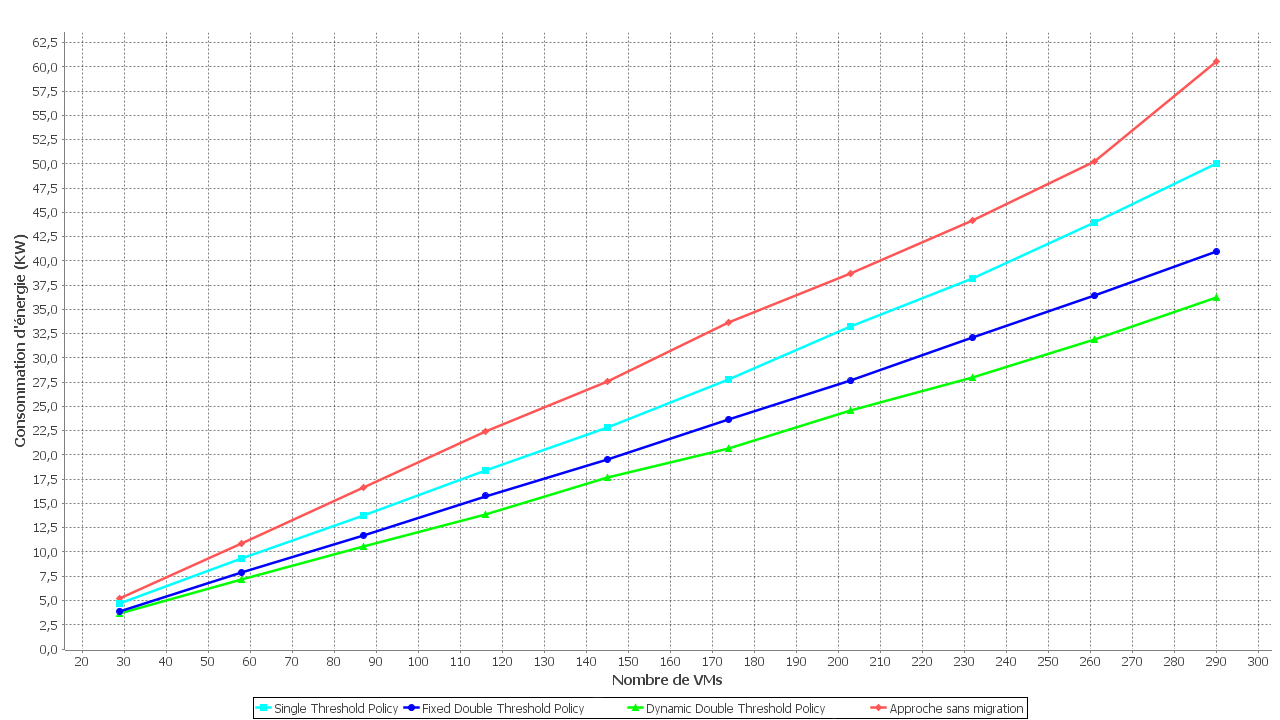
\includegraphics[scale=0.35]{figures/sh1.png} 
\end{center}
\caption{Influence du nombre des VMs sur l’énergie}
\label{InNVMEn}
\end{figure}


\subsubsection{Nombre de migrations}
Dans cette série de simulations représentée par la Figure \ref{InNVMEnM}, nous remarquons  une augmentation du nombre de migrations dans les  trois approches. Nous pouvons justifier cela par l’augmentation du nombre des VMs.
Nous remarquons aussi qu’avec l’augmentation du nombre de VMs, la différence entre les courbes augmente et les courbes des approches proposées se trouvent au-dessous de la courbe de l’approche \textbf{Single Threshold}. Donc les approches \textbf{Fixed Double Threshold} et \textbf{Dynamic Double Threshold} sont bien meilleures que l’approche Single Threshold et permettent de minimiser le nombre de migrations.

Le tableau \ref{tab3} compare entre les trois approches (\textbf{Single Threshold}, \textbf{Fixed Double Threshold} et \textbf{ Dynamic Double Threshold}). Nous remarquons  que les  approches proposées réduisent le nombre de migration des VMs par rapport à l’approche \textbf{single Threshold}.

\begin{center}
{\scriptsize   \begin{tabular}{|p{2.5cm}|c|c|c|c|c|c|c|c|c|c|}
\hline
      \centering     Nombre de VMs &  29& 58& 87& 116& 145& 174& 203& 232& 261& 290\\
\hline
      \centering      Single Threshold &  4589& 10885& 16807& 22970& 29323& 35502& 41896& 48240& 54692& 61072\\
\hline
      \centering      Fixed Double Threshold &  2060& 5638& 10049& 15038& 18630& 25452& 29861& 34003& 40886& 44736\\
\hline
      \centering     Dynamic Double Threshold &  415& 1446& 1976& 2674& 3715& 4363& 5291& 6714& 7448& 9346\\
\hline
\end{tabular}}
\captionof{table}{Comparaison entre le nombre de migrations des trois approches}
\label{tab3}
\end{center}

\begin{figure}[!h]
\begin{center}
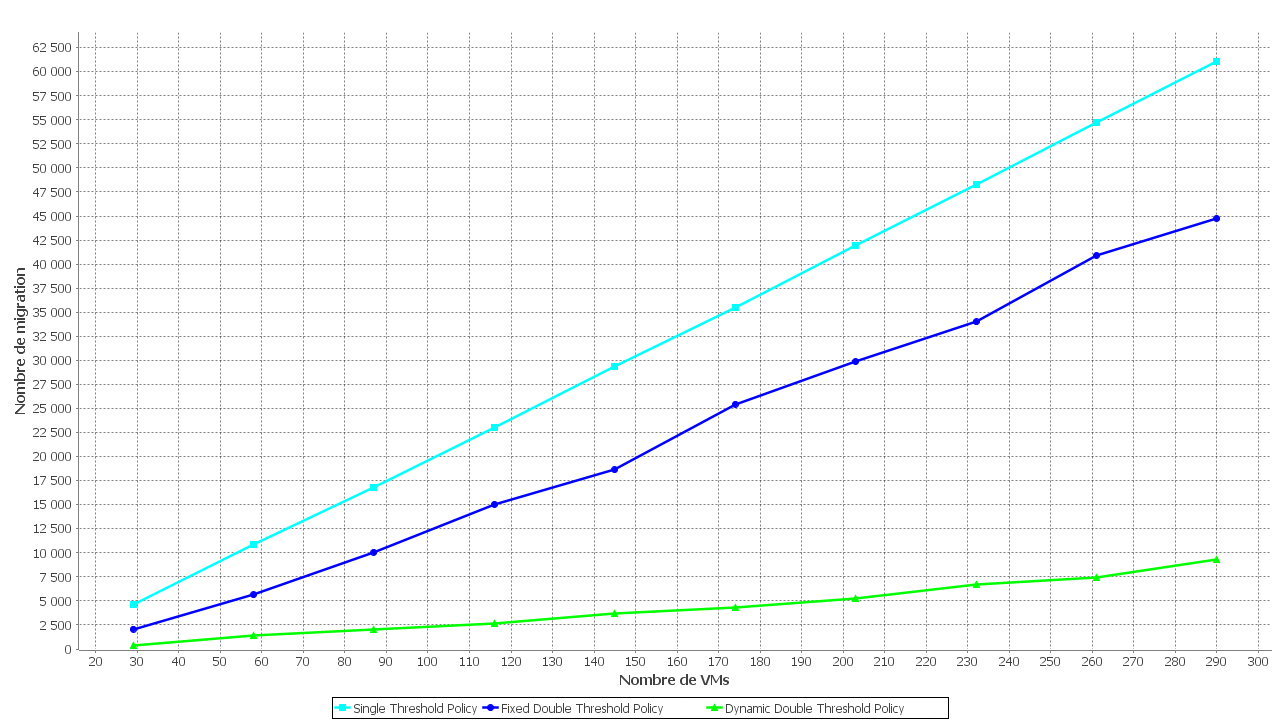
\includegraphics[scale=0.35]{figures/sh2.png} 
\end{center}
\caption{Influence du nombre des VMs sur le nombre de migrations}
\label{InNVMEnM}
\end{figure}

Le tableau \ref{GAIN2} montre la différence entre les trois approches, où nous pouvons déduire que notre approche \textbf{Dynamic Double Threshold} a réduit le nombre de migrations avec un gain moyen de 87,38\% par rapport à l'approche \textbf{Single Threshold} et un gain moyen de 80,31\% par rapport à l'approche \textbf{Fixed Double Threshold}.\\


\begin{center}
{\scriptsize   \begin{tabular}{|p{3.5cm}|c|}
\hline
      \centering      Nom de l’approche &  Gain\\
\hline
      \centering      Single Threshold et Dynamic Double Threshold&  87,38\%\\
\hline
      \centering      Fixed Double Threshold et Dynamic Double Threshold&  80,31\%\\
\hline
\end{tabular}}
\captionof{table}{Comparaison entre le nombre de migrations des trois approches}
\label{GAIN2}
\end{center}

\subsubsection{Violation de SLA}
La Figure \ref{InNVMEV} résultante du tableau \ref{tab4} montre le comportement des deux approches par rapport au nombre de violations de SLA. Nous remarquons que les courbes des approches \textbf{Fixed Double Threshold} et \textbf{Dynamic Double Threshold} se trouvent au-dessous de la courbe de l’approche \textbf{Single Threshold}. Nous remarquons aussi qu’avec l’augmentation du nombre de VMs, la différence entre les courbes augmente. Donc les approches \textbf{Fixed Double Threshold} et \textbf{Dynamic Double Threshold} permettent de minimiser le nombre de violations de SLA.

\begin{center}
{\scriptsize   \begin{tabular}{|p{2.5cm}|c|c|c|c|c|c|c|c|c|c|}
\hline
      \centering     Nombre de VMs &  29& 58& 87& 116& 145& 174& 203& 232& 261& 290\\
\hline
      \centering      Single Threshold &  4786& 12420& 20010& 27810& 36461& 44241& 52839& 61543& 70830& 79590\\
\hline
      \centering      Fixed Double Threshold &  3023& 8827& 16125& 23449& 30604& 40439& 48878& 55547& 67278& 75000\\
\hline
      \centering     Dynamic Double Threshold &  993& 3840& 6402& 8112& 12821& 15182& 17325& 22882& 26316& 29488\\
\hline
\end{tabular}}
\captionof{table}{Comparaison entre le nombre de violations de SLA des trois approches}
\label{tab4}
\end{center}
\clearpage
\begin{figure}[!h]
\begin{center}
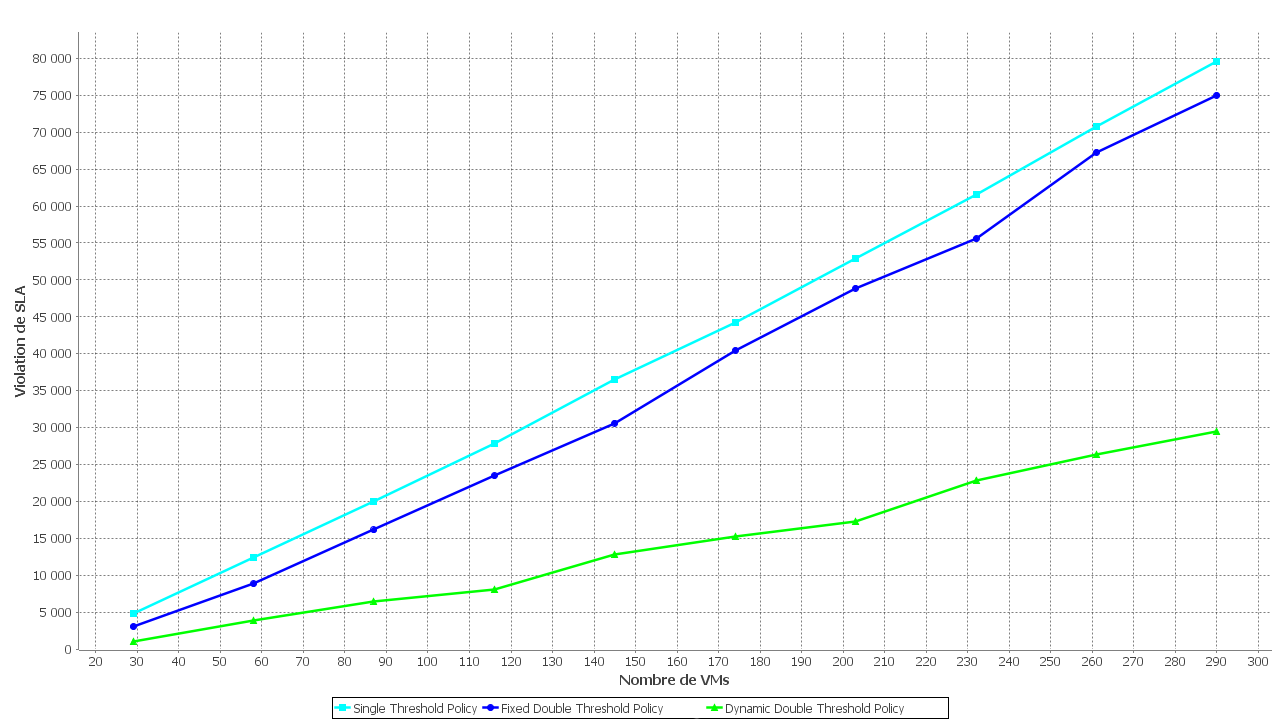
\includegraphics[scale=0.35]{figures/sh3.png} 
\end{center}
\caption{Influence du nombre des VMs sur le nombre de violations de SLA}
\label{InNVMEV}
\end{figure}

Le tableau \ref{GAIN3} montre la différence entre les trois approches, où nous pouvons déduire que notre approche \textbf{Dynamic Double Threshold} a réduit le nombre de violation de SLA avec un gain moyen de 67,35\% par rapport à l'approche \textbf{Single Threshold} et un gain moyen de 61,48\% par rapport à l'approche \textbf{Fixed Double Threshold}.\\


\begin{center}
{\scriptsize   \begin{tabular}{|p{3.5cm}|c|}
\hline
      \centering      Nom de l’approche&  Gain\\
\hline
      \centering      Single Threshold et Dynamic Double Threshold&  67,35\%\\
\hline
      \centering      Fixed Double Threshold et Dynamic Double Threshold&  61,48\%\\
\hline
\end{tabular}}
\captionof{table}{Comparaison entre le nombre de violations de SLA des trois approches}
\label{GAIN3}
\end{center}
Le tableau \ref{PVSLA} montre que l’approche \textbf{Dynamic Double Threshold} a un pourcentage moyen de violation de SLA moins que l’approche \textbf{Single Threshold} et l’approche \textbf{Fixed Double Threshold}.
\begin{center}
{\scriptsize   \begin{tabular}{|p{2.5cm}|c|c|c|c|c|c|c|c|c|c|c|}
\hline
      \centering     Nombre de VMs &  29& 58& 87& 116& 145& 174& 203& 232& 261& 290& Moyen\\
\hline
      \centering      Single Threshold (\%)&  40.83& 41.51& 44.80& 47.39& 48.33& 48.71& 49.33& 49.54& 48.89& 47.81& 46.61\\
\hline
      \centering      Fixed Double Threshold (\%)&  12.92& 17.11& 20.32& 20.48& 22.22& 21.92& 24.41& 25.65& 24.24& 26.82& 21.90\\
\hline
      \centering     Dynamic Double Threshold (\%)&  6.28& 7.37& 7.82& 7.48& 8.57& 8.25& 10.49& 11.40& 10.25& 10.35& 9.12\\
\hline
\end{tabular}}
\captionof{table}{Comparaison entre le pourcentage de violation de SLA des trois approches}
\label{PVSLA}
\end{center}

\subsection{Expérience 2 : Variation du nombre de hôtes}

Pour étudier l’impact du nombre d’hôtes sur la consommation d’énergie, le nombre de migrations et le nombre de violations des SLA, nous avons mesuré les trois principales métriques en appliquant les quatre approches. Nous avons créé un Data Center avec un nombre d’hôtes qui varie de 100 à 280 hôtes avec un pas de 20 où chaque hôte est caractérisée par 1 processeur avec une vitesse variante en MIPS (1000, 2000 ou 3000), 8GB de mémoire, 1TB de stockage et consomme une énergie de 175 W avec 0\% d’utilisation du processeur jusqu’à 250 W avec 100\% d’utilisation du processeur. Le Broker crée pour chaque simulation 290 VMs hétérogènes. Chaque VM possède 1 processeur avec une vitesse variante en MIPS (250, 500, 750 ou 1000), 128MB de mémoire, 1GB de stockage. Nous avons considéré le seuil de l’approche \textbf{Single Threshold} comme 0.6 et les deux seuils supérieur et inférieur de l’approche \textbf{Fixed Double Threshold} comme 0,6 et 0,3 respectivement.


\subsubsection{Consommation d’énergie}
Pour analyser la consommation d’énergie, les résultats obtenus par les simulations sont résumés numériquement dans le tableau \ref{tab5} et schématisés par la Figure \ref{InNVMEn1}. Nous remarquons durant cette série de simulations que les courbes de nos approches se trouvent au-dessous des courbes des autres approches. Donc nos approches sont bien meilleures que  les autres et permettent d’économiser l’énergie consommée.

\begin{center}
{\scriptsize   \begin{tabular}{|p{3.5cm}|c|c|c|c|c|c|c|c|c|c|}
\hline
      \centering     Nombre de PMs &  100& 120& 140& 160& 180& 200& 220& 240& 260& 280\\
\hline
     \centering       Approche sans migration &  35.94& 32.78& 31.34& 30.13& 28.79& 28.68& 28.70& 28.70& 28.67& 28.65\\
\hline
      \centering      Single Threshold &  29.96& 30.10& 28.13& 26.05& 25.37& 24.99& 24.38& 23.84& 23.38& 23.27\\
\hline
      \centering      Fixed Double Threshold &  21.70& 20.57& 19.98& 19.43& 19.13& 19.04& 19.05& 19.06& 19.14& 19.14\\
\hline
      \centering     Dynamic Double Threshold &  17.71& 16.67& 16.60& 16.46& 16.40& 16.39& 16.46& 16.28& 16.42& 16.23\\
\hline
\end{tabular}}
\captionof{table}{Comparaison entre la consommation d’énergie des quatre approches}
\label{tab5}
\end{center}


\begin{figure}[!h]
\begin{center}
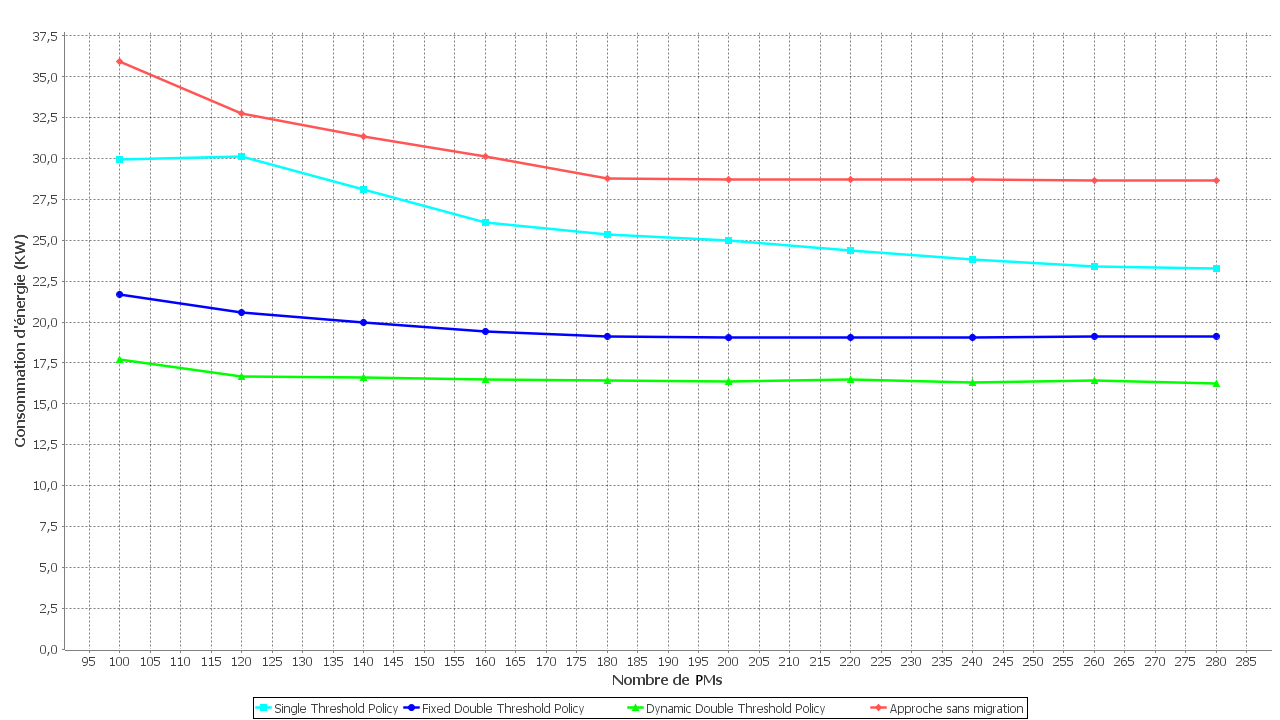
\includegraphics[scale=0.35]{figures/sh4.png} 
\end{center}
\caption{Influence du nombre des PMs sur l’énergie}
\label{InNVMEn1}
\end{figure}

Le tableau \ref{GAIN4} montre la différence entre les quatre approches, où nous pouvons déduire que notre approche \textbf{Dynamic Double Threshold} a réduit l’énergie avec un gain moyen de 45,01\% par rapport à l'approche sans migration, un gain moyen de 35,67\% par rapport à l'approche \textbf{Single Threshold} et un gain moyen de 15,53\% par rapport à l'approche \textbf{Fixed Double Threshold}.\\


\begin{center}
{\scriptsize   \begin{tabular}{|p{3.5cm}|c|}
\hline
      \centering      Nom de l’approche&  Gain\\
\hline
     \centering       Approche sans migration et Dynamic Double Threshold &  45,01\%\\
\hline
      \centering      Single Threshold et Dynamic Double Threshold&  35,67\%\\
\hline
      \centering      Fixed Double Threshold et Dynamic Double Threshold&  15,53\%\\
\hline
\end{tabular}}
\captionof{table}{Comparaison entre la consommation d’énergie des quatre approches}
\label{GAIN4}
\end{center}

\subsubsection{Nombre de migration}
D’après la Figure \ref{InNVMEnM1} et le tableau \ref{tab6}, nous pouvons remarquer que nos approches \textbf{Fixed Double Threshold} et \textbf{Dynamic Double Threshold} ont réduit le nombre de migration par rapport à l’approche \textbf{Single Threshold}.
\begin{center}
{\scriptsize   \begin{tabular}{|p{2.5cm}|c|c|c|c|c|c|c|c|c|c|}
\hline
      \centering     Nombre de PMs & 100& 120& 140& 160& 180& 200& 220& 240& 260& 280\\
\hline
      \centering      Single Threshold &  57883& 61306& 62329& 62475& 62417& 62363& 62432& 62171& 62161& 61992\\
\hline
      \centering      Fixed Double Threshold &  20117& 20269& 20271& 19929& 18984& 19916& 19811& 20009& 19864& 19403\\
\hline
      \centering     Dynamic Double Threshold &  4105& 4273& 3963& 3867& 3937& 3881& 3602& 4222& 4076& 4071\\
\hline
\end{tabular}}
\captionof{table}{Comparaison entre le nombre de migration des quatre approches}
\label{tab6}
\end{center}
\clearpage
\begin{figure}[!h]
\begin{center}
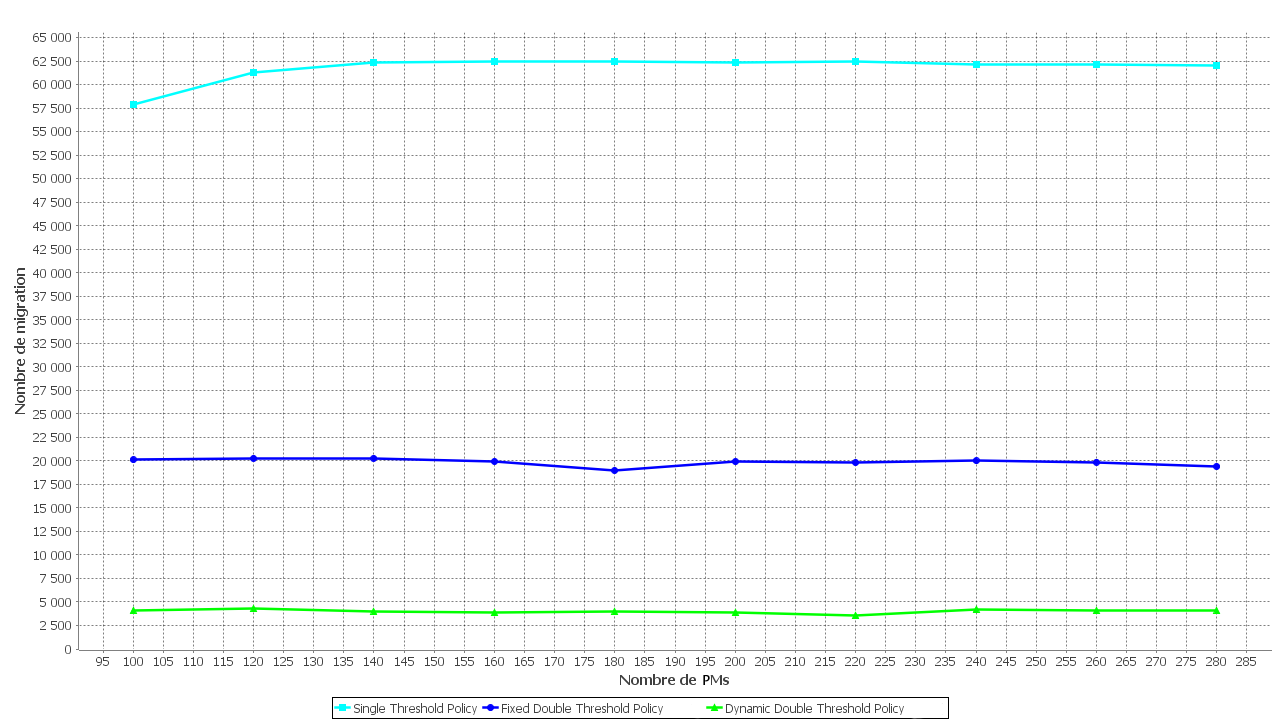
\includegraphics[scale=0.35]{figures/sh5.png} 
\end{center}
\caption{Influence du nombre des PMs sur le nombre de migration}
\label{InNVMEnM1}
\end{figure}


Le tableau \ref{GAIN5} montre la différence entre les trois approches, où nous pouvons déduire que notre approche \textbf{Dynamic Double Threshold} a réduit le nombre de migration avec un gain moyen de 93,51\% par rapport à l'approche \textbf{Single Threshold} et un gain moyen de 79,85\% par rapport à l'approche \textbf{Fixed Double Threshold}.\\

\begin{center}
{\scriptsize   \begin{tabular}{|p{3.5cm}|c|}
\hline
      \centering      Nom de l’approche&  Gain\\
\hline
      \centering      Single Threshold et Dynamic Double Threshold&  93,51\%\\
\hline
      \centering      Fixed Double Threshold et Dynamic Double Threshold&  79,85\%\\
\hline
\end{tabular}}
\captionof{table}{Comparaison entre le nombre de migration des trois approches}
\label{GAIN5}
\end{center}

\subsubsection{Violation de SLA}
La Figure \ref{InNVMEV1} résultante du tableau \ref{tab7} montre que les approches \textbf{Fixed Double Threshold} et \textbf{Dynamic Double Threshold} permettent de minimiser le nombre de violation de SLA par rapport à l’approche \textbf{Single Threshold}.

\begin{center}
{\scriptsize   \begin{tabular}{|p{2.5cm}|c|c|c|c|c|c|c|c|c|c|}
\hline
      \centering     Nombre de PMs &  100& 120& 140& 160& 180& 200& 220& 240& 260& 280\\
\hline
      \centering      Single Threshold &  62422& 63861& 64238& 64087& 64043& 63792& 64065& 63723& 63669& 63346\\
\hline
      \centering      Fixed Double Threshold &  33563& 33200& 32658& 32385& 31741& 32394& 32847& 32401& 32396& 31655\\
\hline
      \centering     Dynamic Double Threshold &  12025& 12637& 11739& 11237& 10863& 11062& 10237& 12238& 11834& 11832\\
\hline
\end{tabular}}
\captionof{table}{Comparaison entre le nombre de violations de SLA des quatre approches}
\label{tab7}
\end{center}

\begin{figure}[!h]
\begin{center}
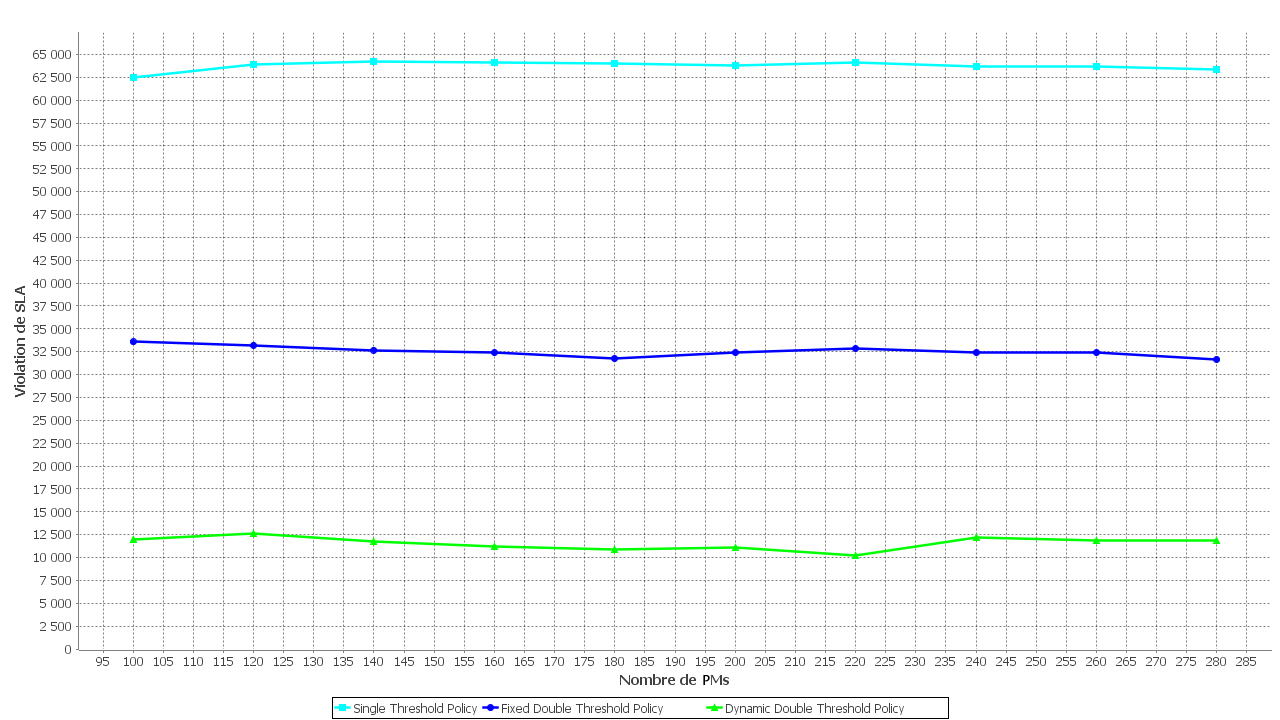
\includegraphics[scale=0.35]{figures/sh6.png} 
\end{center}
\caption{Influence du nombre des PMs sur le nombre de violations de SLA}
\label{InNVMEV1}
\end{figure}

Le tableau \ref{GAIN6} montre la différence entre les trois approches, où nous pouvons déduire que notre approche \textbf{Dynamic Double Threshold} a réduit le nombre de violation de SLA avec un gain moyen de 81,83\% par rapport à l'approche \textbf{Single Threshold} et un gain moyen de 64,42\% par rapport à l'approche \textbf{Fixed Double Threshold}.\\ 
\begin{center}
{\scriptsize   \begin{tabular}{|p{3.5cm}|c|}
\hline
      \centering      Nom de l’approche&  Gain\\
\hline
      \centering      Single Threshold et Dynamic Double Threshold&  81,83\%\\
\hline
      \centering      Fixed Double Threshold et Dynamic Double Threshold&  64,42\%\\
\hline
\end{tabular}}
\captionof{table}{Comparaison entre le nombre de violation de SLA des trois approches}
\label{GAIN6}
\end{center}

Le tableau \ref{PVSLA2} montre que l’approche \textbf{Dynamic Double Threshold} a un pourcentage moyen de violation de SLA moins que l’approche \textbf{Single Threshold} et l’approche \textbf{Fixed Double Threshold}.

\begin{center}
{\scriptsize   \begin{tabular}{|p{2.5cm}|c|c|c|c|c|c|c|c|c|c|c|}
\hline
      \centering     Nombre de PMs &  100& 120& 140& 160& 180& 200& 220& 240& 260& 280& \\
\hline
      \centering      Single Threshold &  47.81& 49.74& 49.87& 50.16& 49.99& 49.87& 49.58& 49.80& 49.55& 49.68& 49.60\\
\hline
      \centering      Fixed Double Threshold &  26.82& 25.29& 25.08& 24.33& 24.92& 25.04& 25.57& 24.87& 25.75& 26.18& 25.21\\
\hline
      \centering     Dynamic Double Threshold &  9.60& 10.00& 9.60& 10.17& 9.70& 9.68& 8.83& 9.90& 9.39& 9.77& 9.66\\
\hline
\end{tabular}}
\captionof{table}{Comparaison entre le pourcentage de violation de SLA des trois approches}
\label{PVSLA2}
\end{center}

\end{onehalfspace}

\section{Conclusion}

\begin{onehalfspace}


Dans ce chapitre, nous avons présenté l’implémentation de notre application ainsi que les résultats obtenus. Aussi, nous avons réalisé plusieurs séries de simulations dans le but de comparer nos approches avec l’approche sans migration et l’approche  \textbf{Single Threshold}   tout en variant différents paramètres comme : le nombre d'hôtes, le nombre de VM. Les résultats de la comparaison ont montré que notre approche permet de minimiser  la consommation d’énergie du système, réduire le nombre de migrations des VMs et par conséquence réduire  le nombre de violations de SLA.

\end{onehalfspace}
\clearpage
\thispagestyle{empty}
\begin{center}
\resizebox{!}{8mm}{\bf \scshape \selectfont Conclusion générale}\\
\end{center}
%\lhead{\normalsize \bf \selectfont Introduction générale}
\vspace{20mm}

%\lipsum[1-3]
\begin{onehalfspace}
\lettrine[nindent=1em,lines=3]{L}e cloud computing est en pleine expansion et tend à s'imposer comme un des paradigmes dominants dans l'univers informatique. Les infrastructures proposant des services de cloud computing deviennent donc de plus en plus nombreuses, et de plus en plus complexes pour répondre à cette demande croissante de services décentralisés. Cette augmentation amène bien évidemment divers problèmes, dont celui de la consommation d'énergie. Il faut donc concevoir des techniques et outils afin de répondre à ces nouveaux besoins de gestion.\\

La migration des machines virtuelles est une technique qui permet de régler en général certains problèmes dans le Cloud tels que les problèmes de la consommation d'énergie.\\

Cette technique consiste à déplacer une machine virtuelle d'un nœud à un autre dont le but d'augmenter considérablement le taux d'utilisation et réduire la consommation d'énergie selon certains critères.\\

Au cours de ce projet, nous avons développé une stratégie pour bien améliorer l'efficacité énergétique dans le Cloud Computing. Nous avons proposé une approche qui se base sur le mécanisme de la migration des machines virtuelles, tout en appliquant certaines méthodes. Et afin de mettre en évidence l'approche proposée, nous avons réalisé plusieurs séries d'expérimentations en faisant varier plusieurs paramètres. Nous avons utilisé, également, les trois principales métriques qui sont l'énergie consommée, nombre de migrations et violations de SLA Sur le plan d'expérimentation, nous avons positionné et comparé nos propositions par rapport à l'approche sans migration  et à l'approche \textit{Single Threshold}.
\clearpage
\textbf{\scshape Perspectives}\\\\
Pour une continuation de notre travail, plusieurs perspectives peuvent être envisagées :
\begin{enumerate}
\item Ajouter un seuil de température afin de limiter  la chaleur dégagée des machines physiques et de minimiser l'énergie consommée des serveurs et des systèmes de refroidissement.
\item Étudier l'influence des systèmes de climatisation des data center sur leur efficacités et leur performances.
\item Implémenter les deux approches proposées dans un environnement de Cloud réel.
\item En plus de l'utilisation du processeur,  prendre en considération   plusieurs ressources au niveau de la phase de migration tels que: la capacité de la RAM, la capacité de stockage et la bande passante. 
\end{enumerate}

\end{onehalfspace}

\listoffigures
\listoftables
\listofalgorithms
\bibliographystyle{alpha} % Le style est mis entre accolades.
%\bibliographystyle{abbrv}
\bibliography{bibli/bibli} % mon fichier de base de données s'appelle bibli.bib
    
%\renewcommand{\thefootnote}{\Alph{footnote}}

\end{document}